\documentclass[11pt, a4paper]{article}
%\usepackage{proj1}
\usepackage{natbib}
\usepackage{fancyhdr}  
\usepackage{subcaption}
\usepackage{caption}
\usepackage{graphicx}
\usepackage{numprint}
\usepackage{multirow}
\linespread{1.25} 
\setlength{\parindent}{0cm}
\graphicspath{{Images/}}
\usepackage{hyperref}
\usepackage{amsmath}
\usepackage{amsfonts}
\usepackage{amssymb}
\usepackage{amsthm}
\usepackage{mathtools}
\usepackage{commath}
\usepackage{bbm}

%\usepackage[sc,osf]{mathpazo}
\usepackage{subcaption}
\usepackage[a4paper, top=1in, left=1.0in, right=1.0in, bottom=1in, includehead, includefoot]{geometry} %Usually have top as 1in

\usepackage{listings}
\usepackage{color} %red, green, blue, yellow, cyan, magenta, black, white
\definecolor{mygreen}{RGB}{28,172,0} % color values Red, Green, Blue
\definecolor{mylilas}{RGB}{170,55,241}


\hypersetup{colorlinks,linkcolor={black},citecolor={blue},urlcolor={black}}
\usepackage{color}
\urlstyle{same}


\theoremstyle{definition}
\newtheorem{definition}{Definition}[section]

%\newcommand{\Sta}{\rho}
\newcommand{\adja}{q_a}
\newcommand{\adjb}{q_b}
\newcommand{\adjaB}{q_{a,\partial \Omega}}
\newcommand{\adjbB}{q_{b,\partial \Omega}}
%\newcommand{\Con}{u}
\newcommand{\ra}{\rho_a}
\newcommand{\rb}{\rho_b}
\newcommand{\w}{\mathbf{w}}
\newcommand{\Stav}{\mathbf{v}}
\newcommand{\Adja}{\mathbf{p}}
\newcommand{\Adjb}{q}
\newcommand{\Adjc}{{p}_{\partial \Sigma}}
\newcommand{\Con}{\mathbf{f}}
\newcommand{\n}{\mathbf{n}}
\newcommand{\h}{\mathbf{h}}
\newcommand{\K}{\mathbf{K}}


\pagenumbering{gobble}
\begin{document}
	\section*{Sedimentation}
	We are interested in modelling sedimentation processes. In order to achieve this, the current equations have to be modified slightly to include an approximation to volume exclusion. This work aims to replicate some of the results achieved in the paper by Archer, referenced below.
	From the paper, we have the following set of equations modelling the sedimentation process:
	\begin{align*}
		&\frac{\partial \rho}{\partial t} = \Gamma\nabla \cdot \left(  \rho \nabla \frac{\delta F[\rho]}{\delta \rho} \right) ,
	\end{align*}
	where $\Gamma$ is the diffusion coefficient. 	
	We can rescale this equation as done in the paper using the relationship $t^* = t/ \tau_B$, where $\tau_B = \beta \sigma^2 / \Gamma$.
	Applying this rescaling (and setting $\beta = 1$ throughout) we get:
	\begin{align}\label{Eq1}
		&\frac{\partial \rho}{\partial t^*} = \sigma^2\nabla \cdot \left(  \rho \nabla \frac{\delta F[\rho]}{\delta \rho} \right) ,
	\end{align}
   The free energy functional is:
		\begin{align*}
		F[\rho] &= \frac{1}{\beta} \int \rho (\ln \Lambda^2 \rho) - 2 \rho - \rho \ln(1 - \eta) + \frac{\rho}{1 - \eta} dr\\
		&+ \frac{1}{2}\int \int \rho(r) \rho(r') V_2(|r - r'|) dr dr' + \int \rho V_{ext} dr,
	\end{align*}
	where $\eta = a \rho = \frac{\pi \sigma^2}{4} \rho$ and the external potential:
	\begin{align*}
			V_{ext} &= a y, \quad \text{for } \quad 0 < y < L,
	\end{align*}
    where $	a = m_B g \sin \theta$ and $L$ is the height of the box. Outside these bounds $V_{ext} = \infty$. 
    Furthermore, we have the pair potential:
	\begin{align*}
		V_2 = - \epsilon exp(-r/\sigma),
	\end{align*}
	where $\sigma$ is the particle diameter of the hard sphere particle and $\epsilon$ the interaction strength.
	We have $L_y = 43.5 \sigma$, and $L_x = 60 \sigma$ from the graphs. 
	We then have the strength of the external potential given by $\beta a = 0.1$ and the strength of the interaction term $\epsilon$ is given by $\beta \epsilon = 3.5$, where $\beta = \frac{1}{k_BT}$. 
	Furthermore, we have the average density of the system $\bar \rho \sigma^2$, calculated using $(1/L_y)\int_0^L \rho \sigma^2 dy$.
	The initial condition for $\rho$ is found by considering $\bar \rho$ and adding a uniform random number to each location in the range $\pm \bar \rho/ 20$. The paper considers the case $\sigma \bar \rho = 0.072$ and $\sigma \bar \rho = 0.2$.
	\section{Replicating examples from the paper in a box with noflux BCs}
	Note that in this section we haven't applied the rescaling with $\sigma^2$ from Equation \eqref{Eq1} and so we cannot compare the time scale here with the one from the paper when considering $\sigma \neq 1$.
	\subsection{Example Figure 8}

	For simplicity, set $\beta = 1$ everywhere. Then set $\sigma = 1$, which gives for the example in Figure 8 that $\bar \rho = 0.072$. However, the domain is rescaled, such that $L_y = 21$, $L_x = 30$ but $\bar \rho = 0.072$. We further have $\epsilon = 3.5$, $a = 0.1$
	The number of points are $n = 30$, $N = 40$ and we run this up to time $T = 30$. If we were to instead increase the strength of $V_{ext}$, we would see the sediment flatten out more at the bottom. The result, which takes $12$ seconds to run, can be seen in Figure \ref{F1}. 
	\begin{figure}[h]
		\centering
		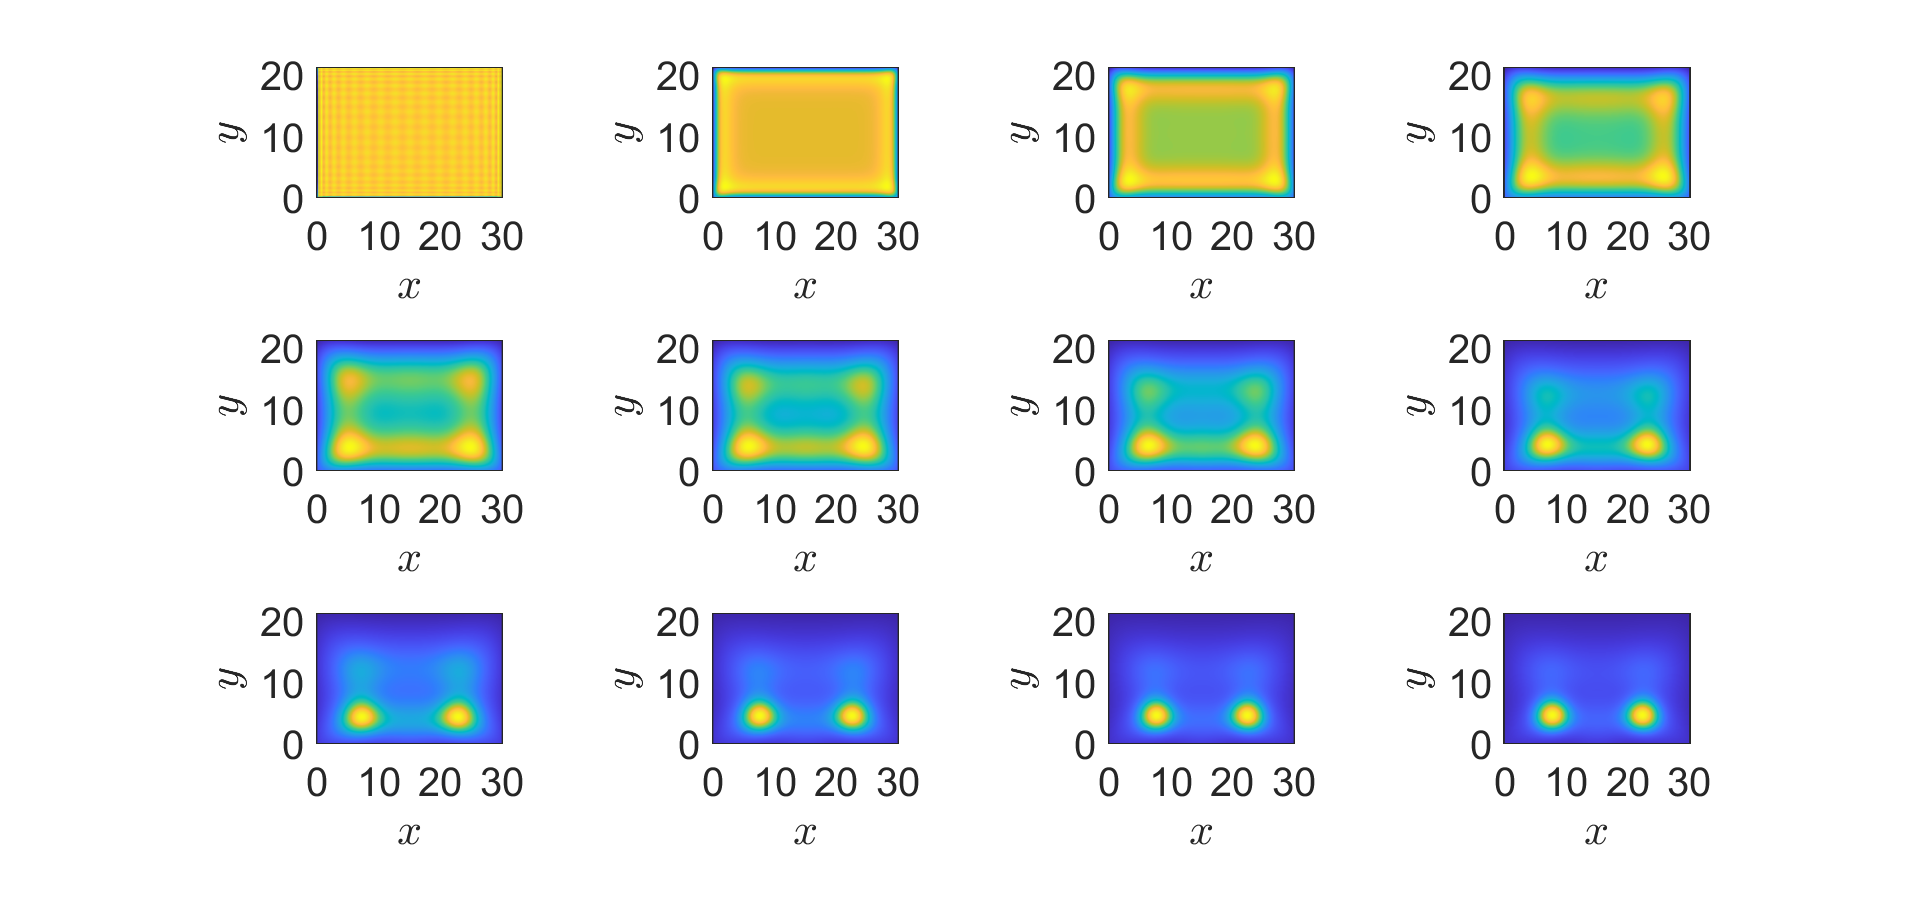
\includegraphics[scale=0.35]{Ex8F1.png}
		\caption{Figure 8 Example, $\bar \rho = 0.072$, $\sigma = 1$, $12$ different times} 
		\label{F1}
	\end{figure} 
	
	
	
	Next, we decrease $\sigma$ to get closer to the scaling from the paper. We set $\sigma = 0.8$. Inspecting the result, it is clear that it needs more points, so we run it with $N = 50$ instead. This increases running time from $30$ seconds to $2$ min. In Figure \ref{F2} we can see that a third cluster is building. 
	\begin{figure}[h]
		\centering
		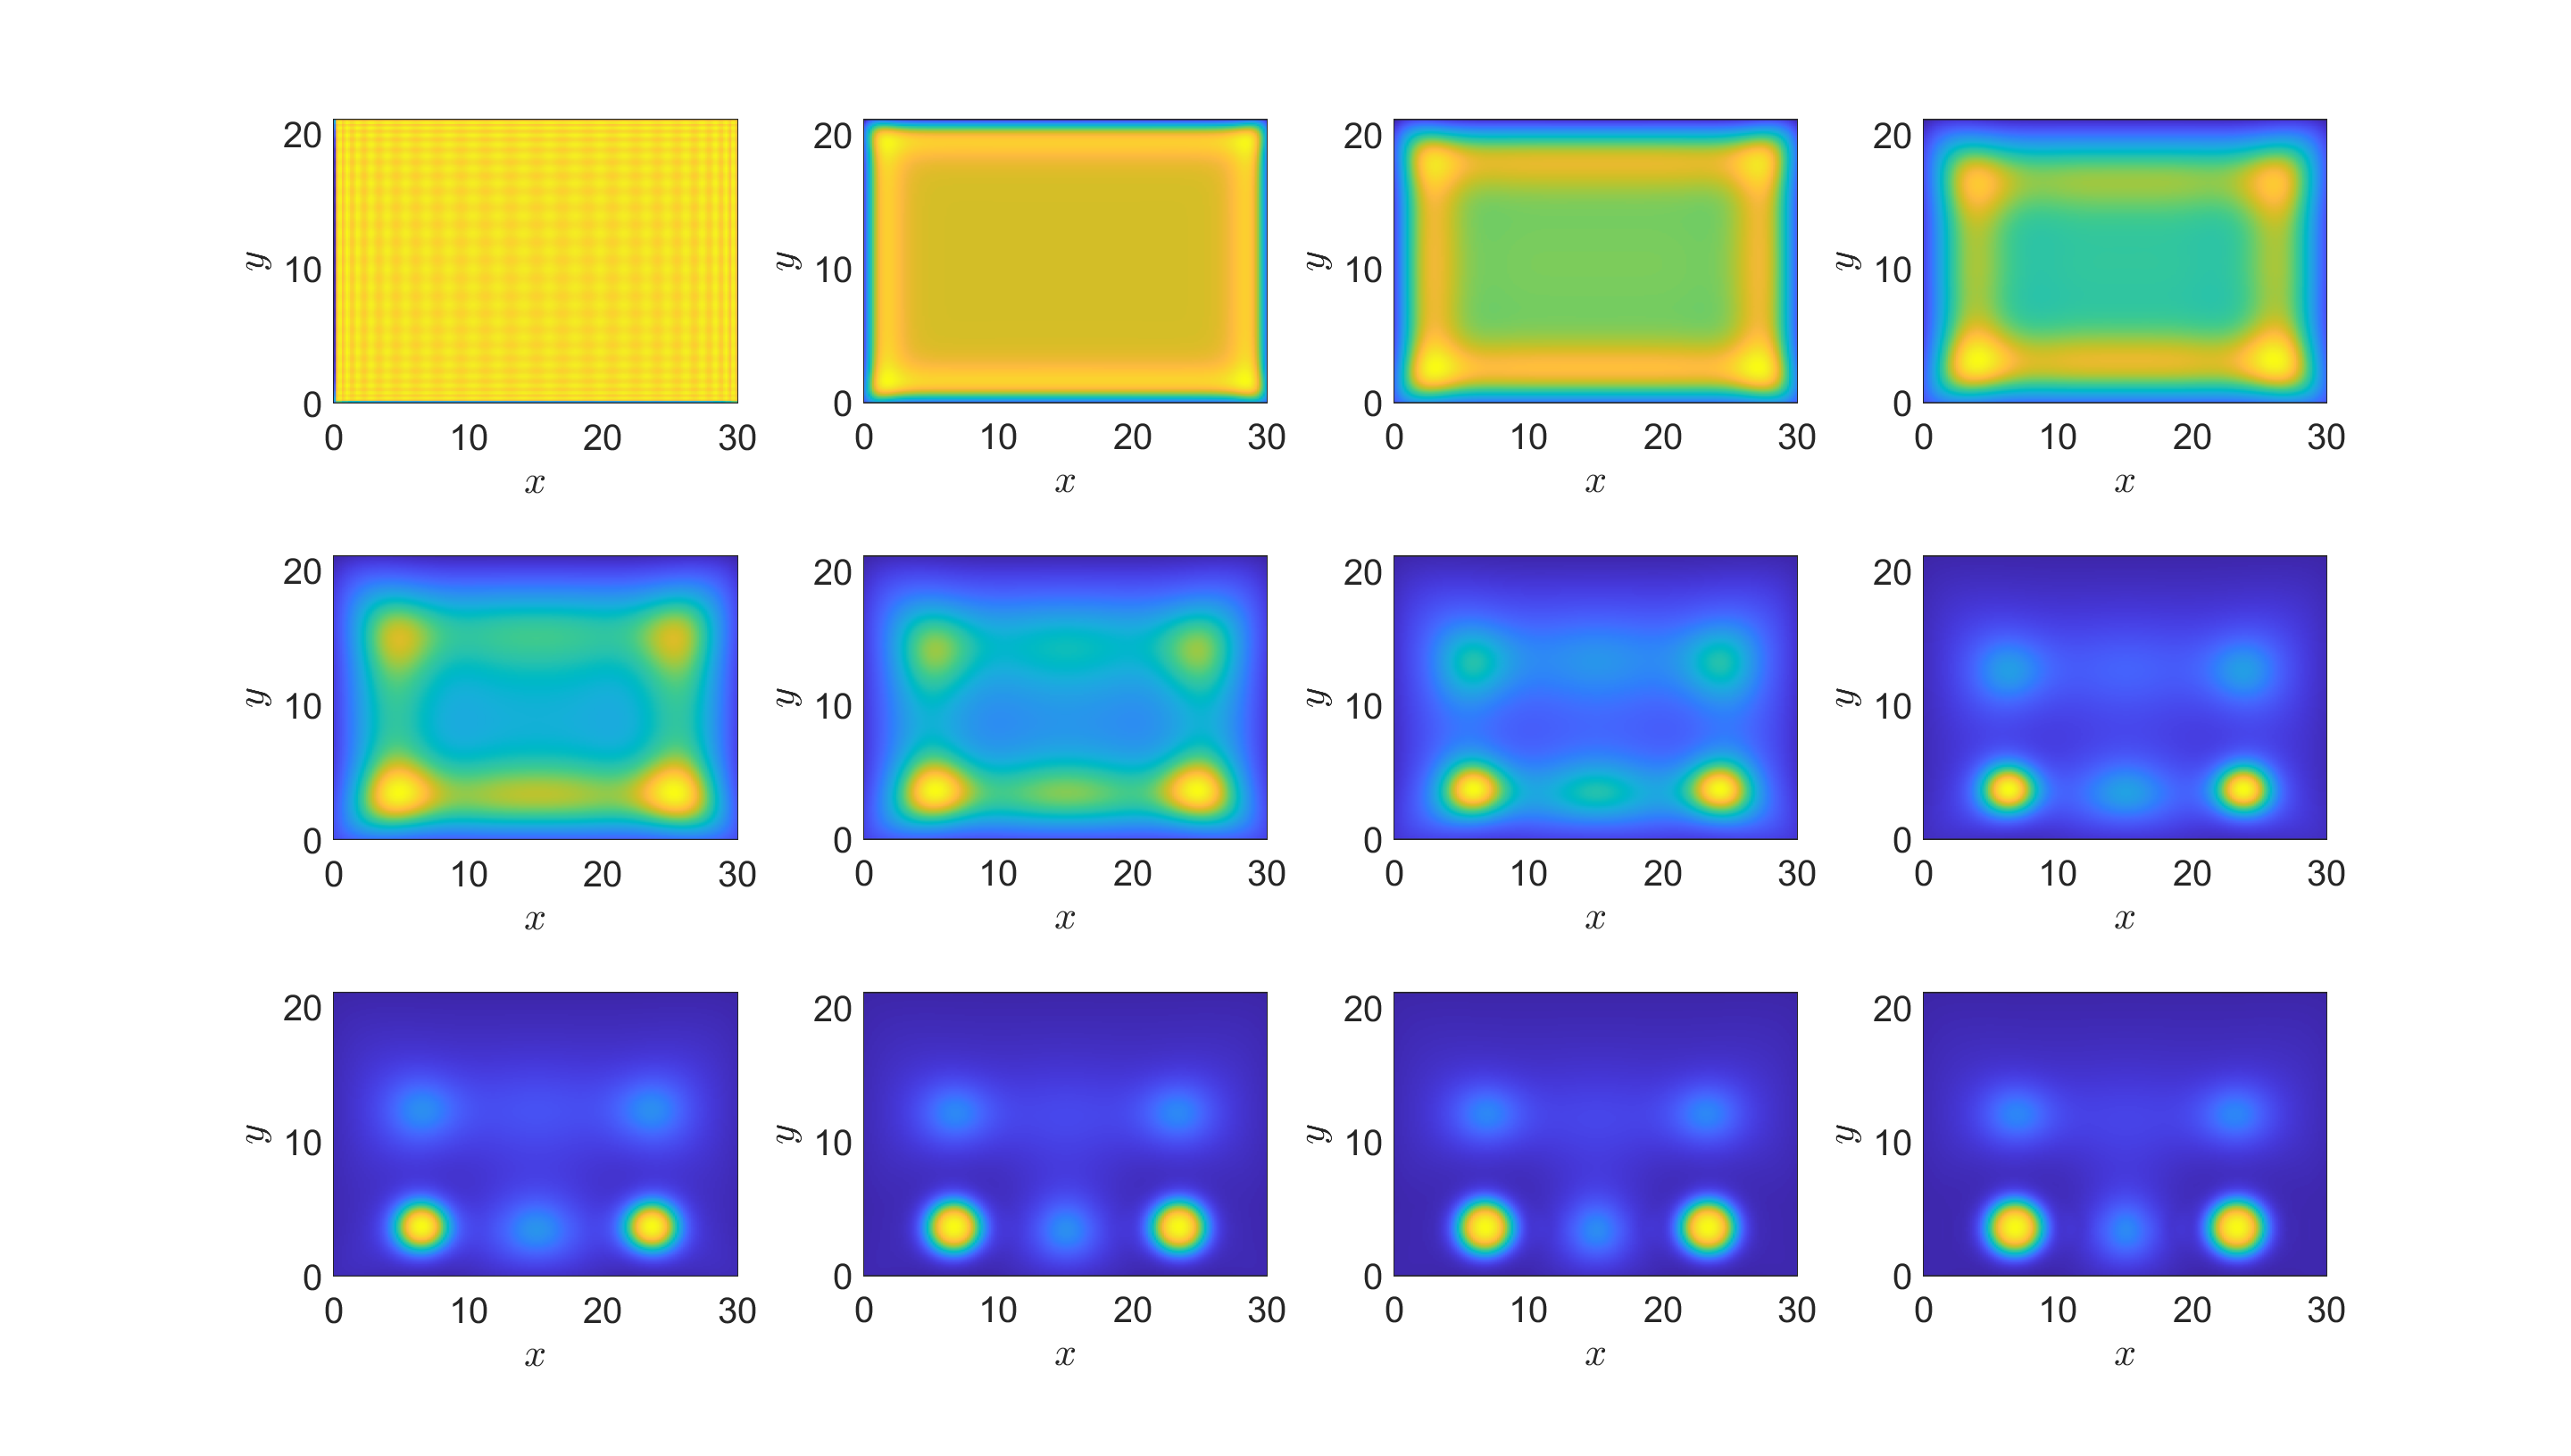
\includegraphics[scale=0.25]{Ex8F2.png}
		\caption{Figure 8 Example, $\bar \rho = 0.072$, $\sigma = 0.8$, $12$ different times} 
		\label{F2}
	\end{figure} 
	 If we decrease $\sigma$ to $0.6$ we again need more points. We try $N = 60$, which takes $14$ min, but the result is still numerically unstable. This can be seen in Figure \ref{F3}.This configuration is closest to the actual model setup because we have half of the domain that Archer has, so we need to half $\sigma$.
	\begin{figure}[h]
		\centering
		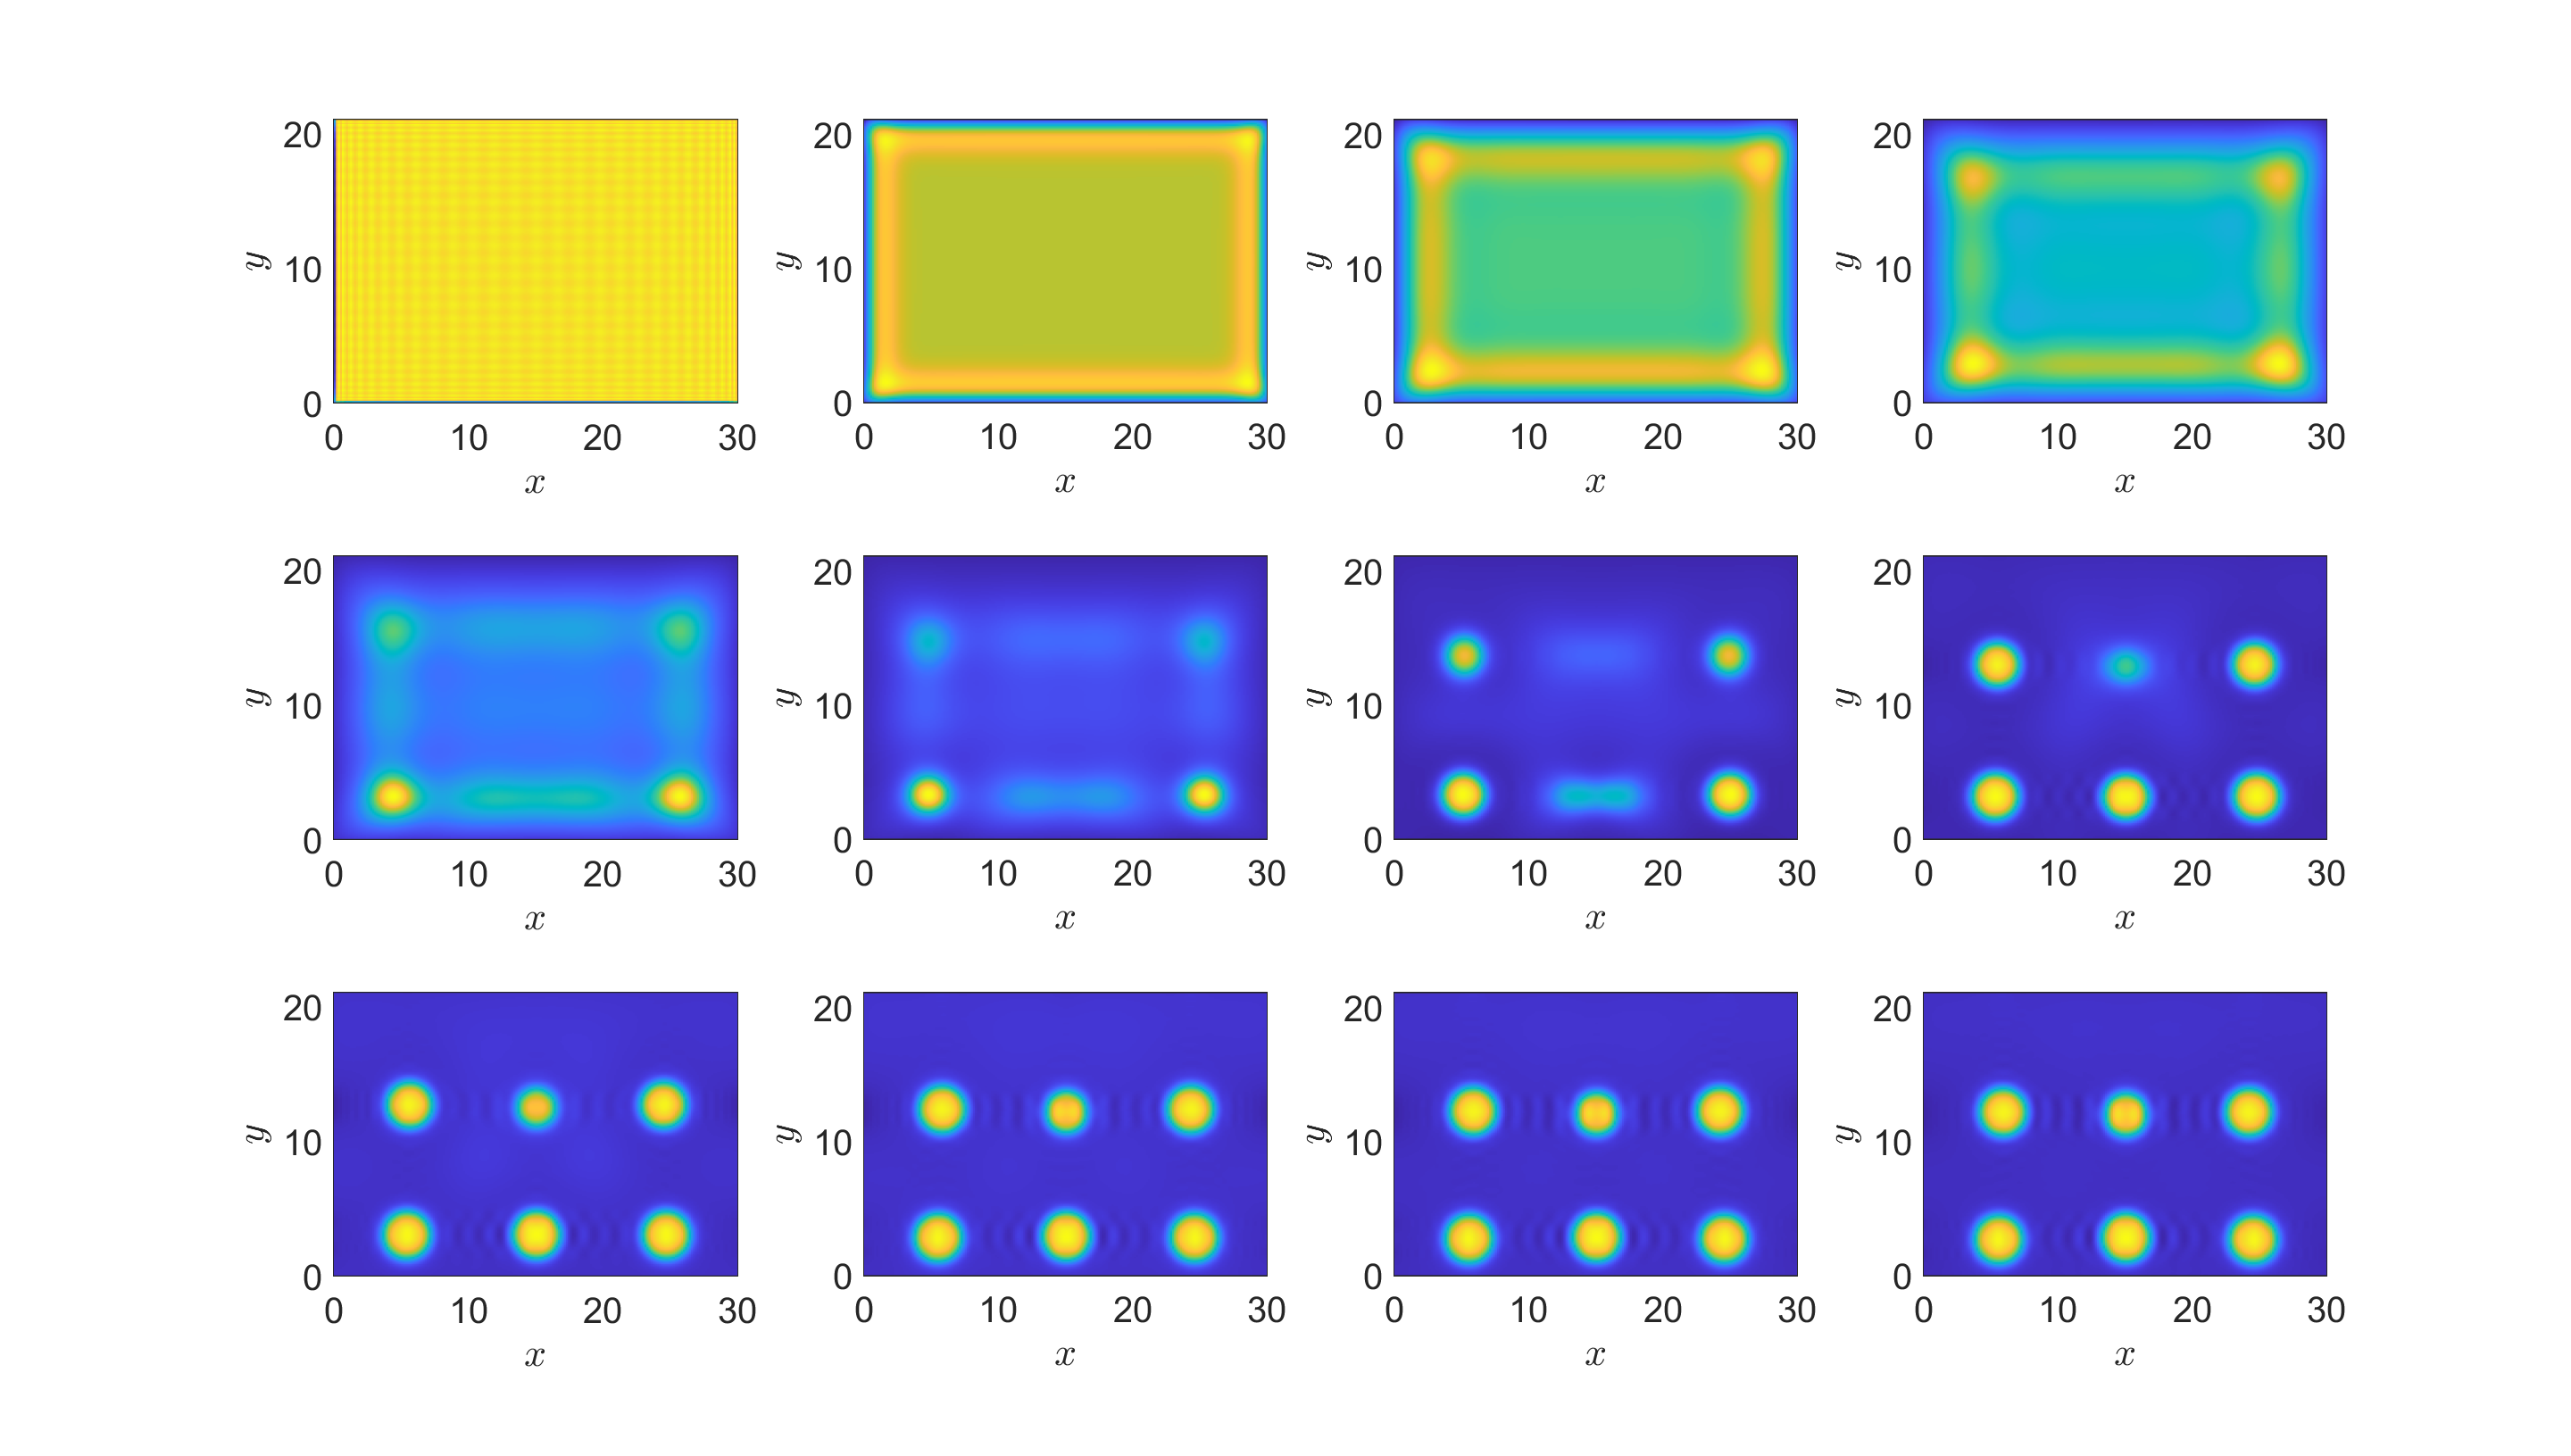
\includegraphics[scale=0.25]{Ex8F3.png}
		\caption{Figure 8 Example, $\bar \rho = 0.072$, $\sigma = 0.5$, $12$ different times} 
		\label{F3}
	\end{figure} 
	
	
	\begin{figure}[h]
		\centering
		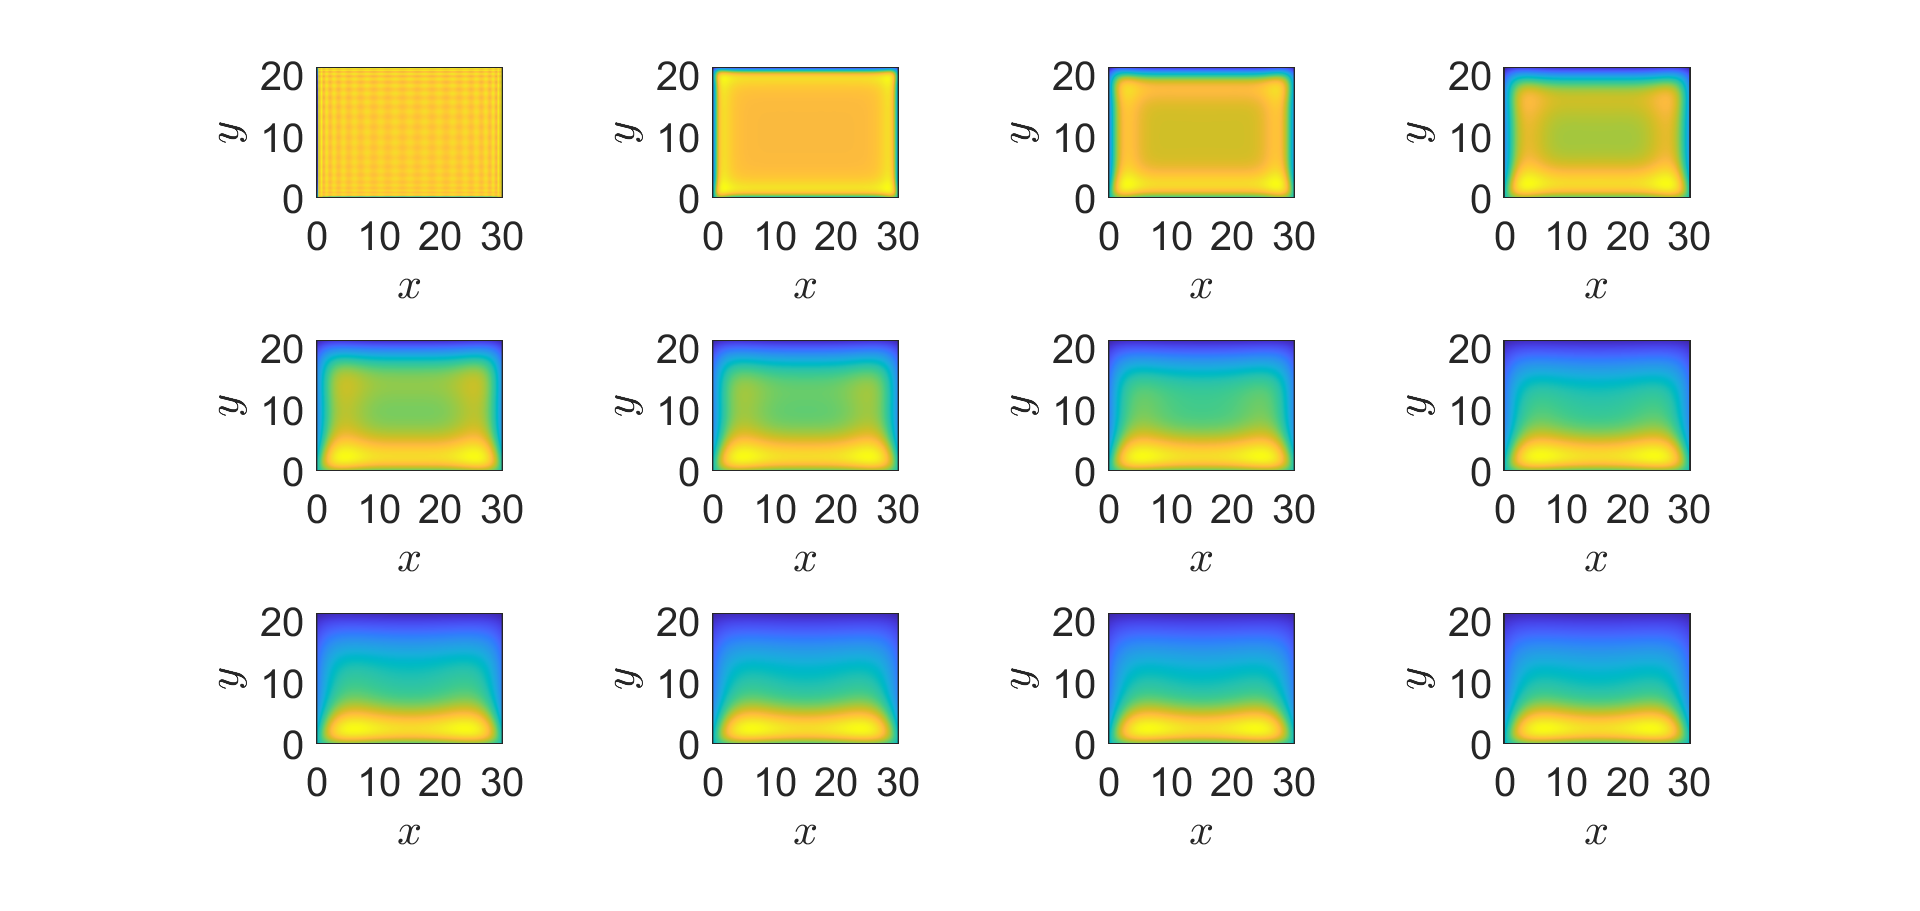
\includegraphics[scale=0.35]{Ex8F1b.png}
		\caption{Figure 8 Example, $\bar \rho = 0.036$, $\sigma = 1$, $12$ different times} 
		\label{F1b}
	\end{figure}
	If I instead decrease $\bar \rho$  to $0.036$, the sediment is more spread out at the bottom.
	
	I then change the initial condition to be non-symmetric: $\bar \rho = 0.072 (1 + \cos(\pi / 30 y_1)\cos(\pi / 30 y_2))$. This has the effect that the final distribution is asymmetric as well, see Figure \ref{Fx}. This is done with $N = 40$, which is again not quite enough for numerical stability, but it takes $1$ min $20$ seconds to solve.
	\begin{figure}[h]
		\centering
		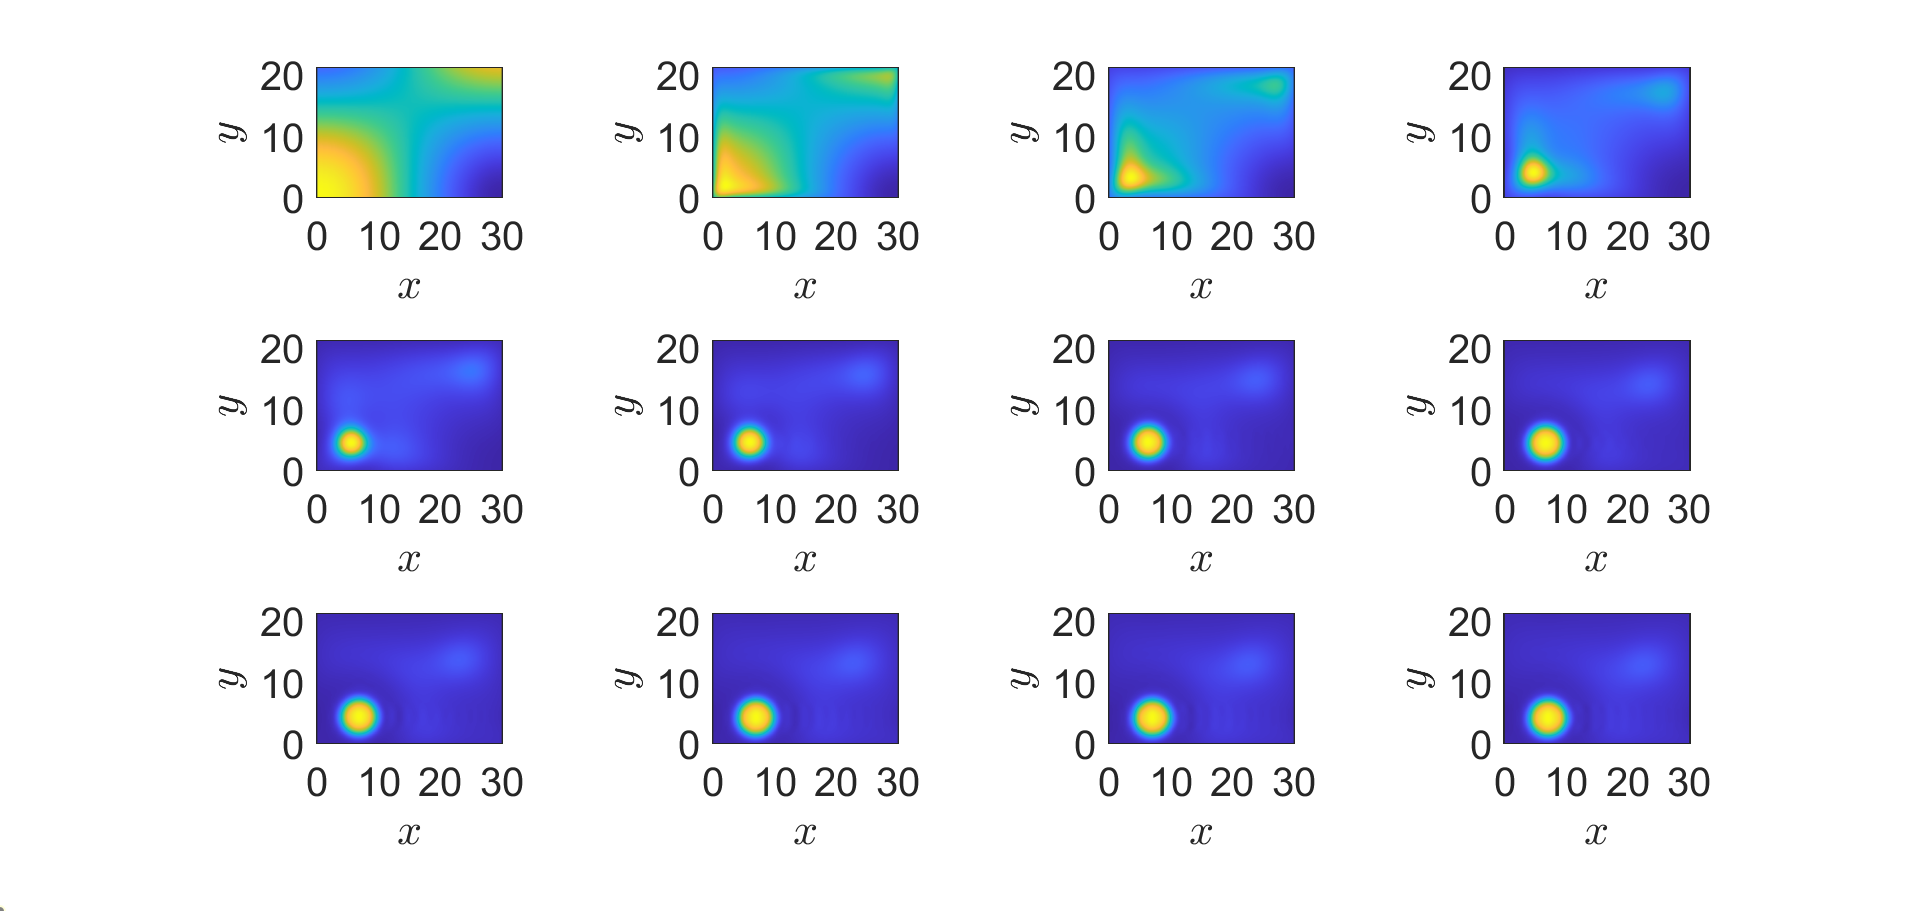
\includegraphics[scale=0.4]{Ex8NonSym.png}
		\caption{Figure 8 Example, $\bar \rho = 0.072$, $\sigma = 1$, $12$ different times, asymmetric initial condition} 
		\label{Fx}
	\end{figure}
	\subsection{Example Figure 10}
	In this example everything stays the same except that more density is in the system, $\bar \rho \sigma^2 = 0.2$. We start with $\sigma = 1$ and $\bar \rho = 0.2$, which needs more points for numerical stability. We try $N = 50$. This is still not quite enough but better and takes $8$ minutes to solve, see Figure \ref{F4}. We can see the sort of behaviour that is visible in the paper, that the different clusters merge. I think if we let time run longer it'd merge into one.
	\begin{figure}[h]
		\centering
		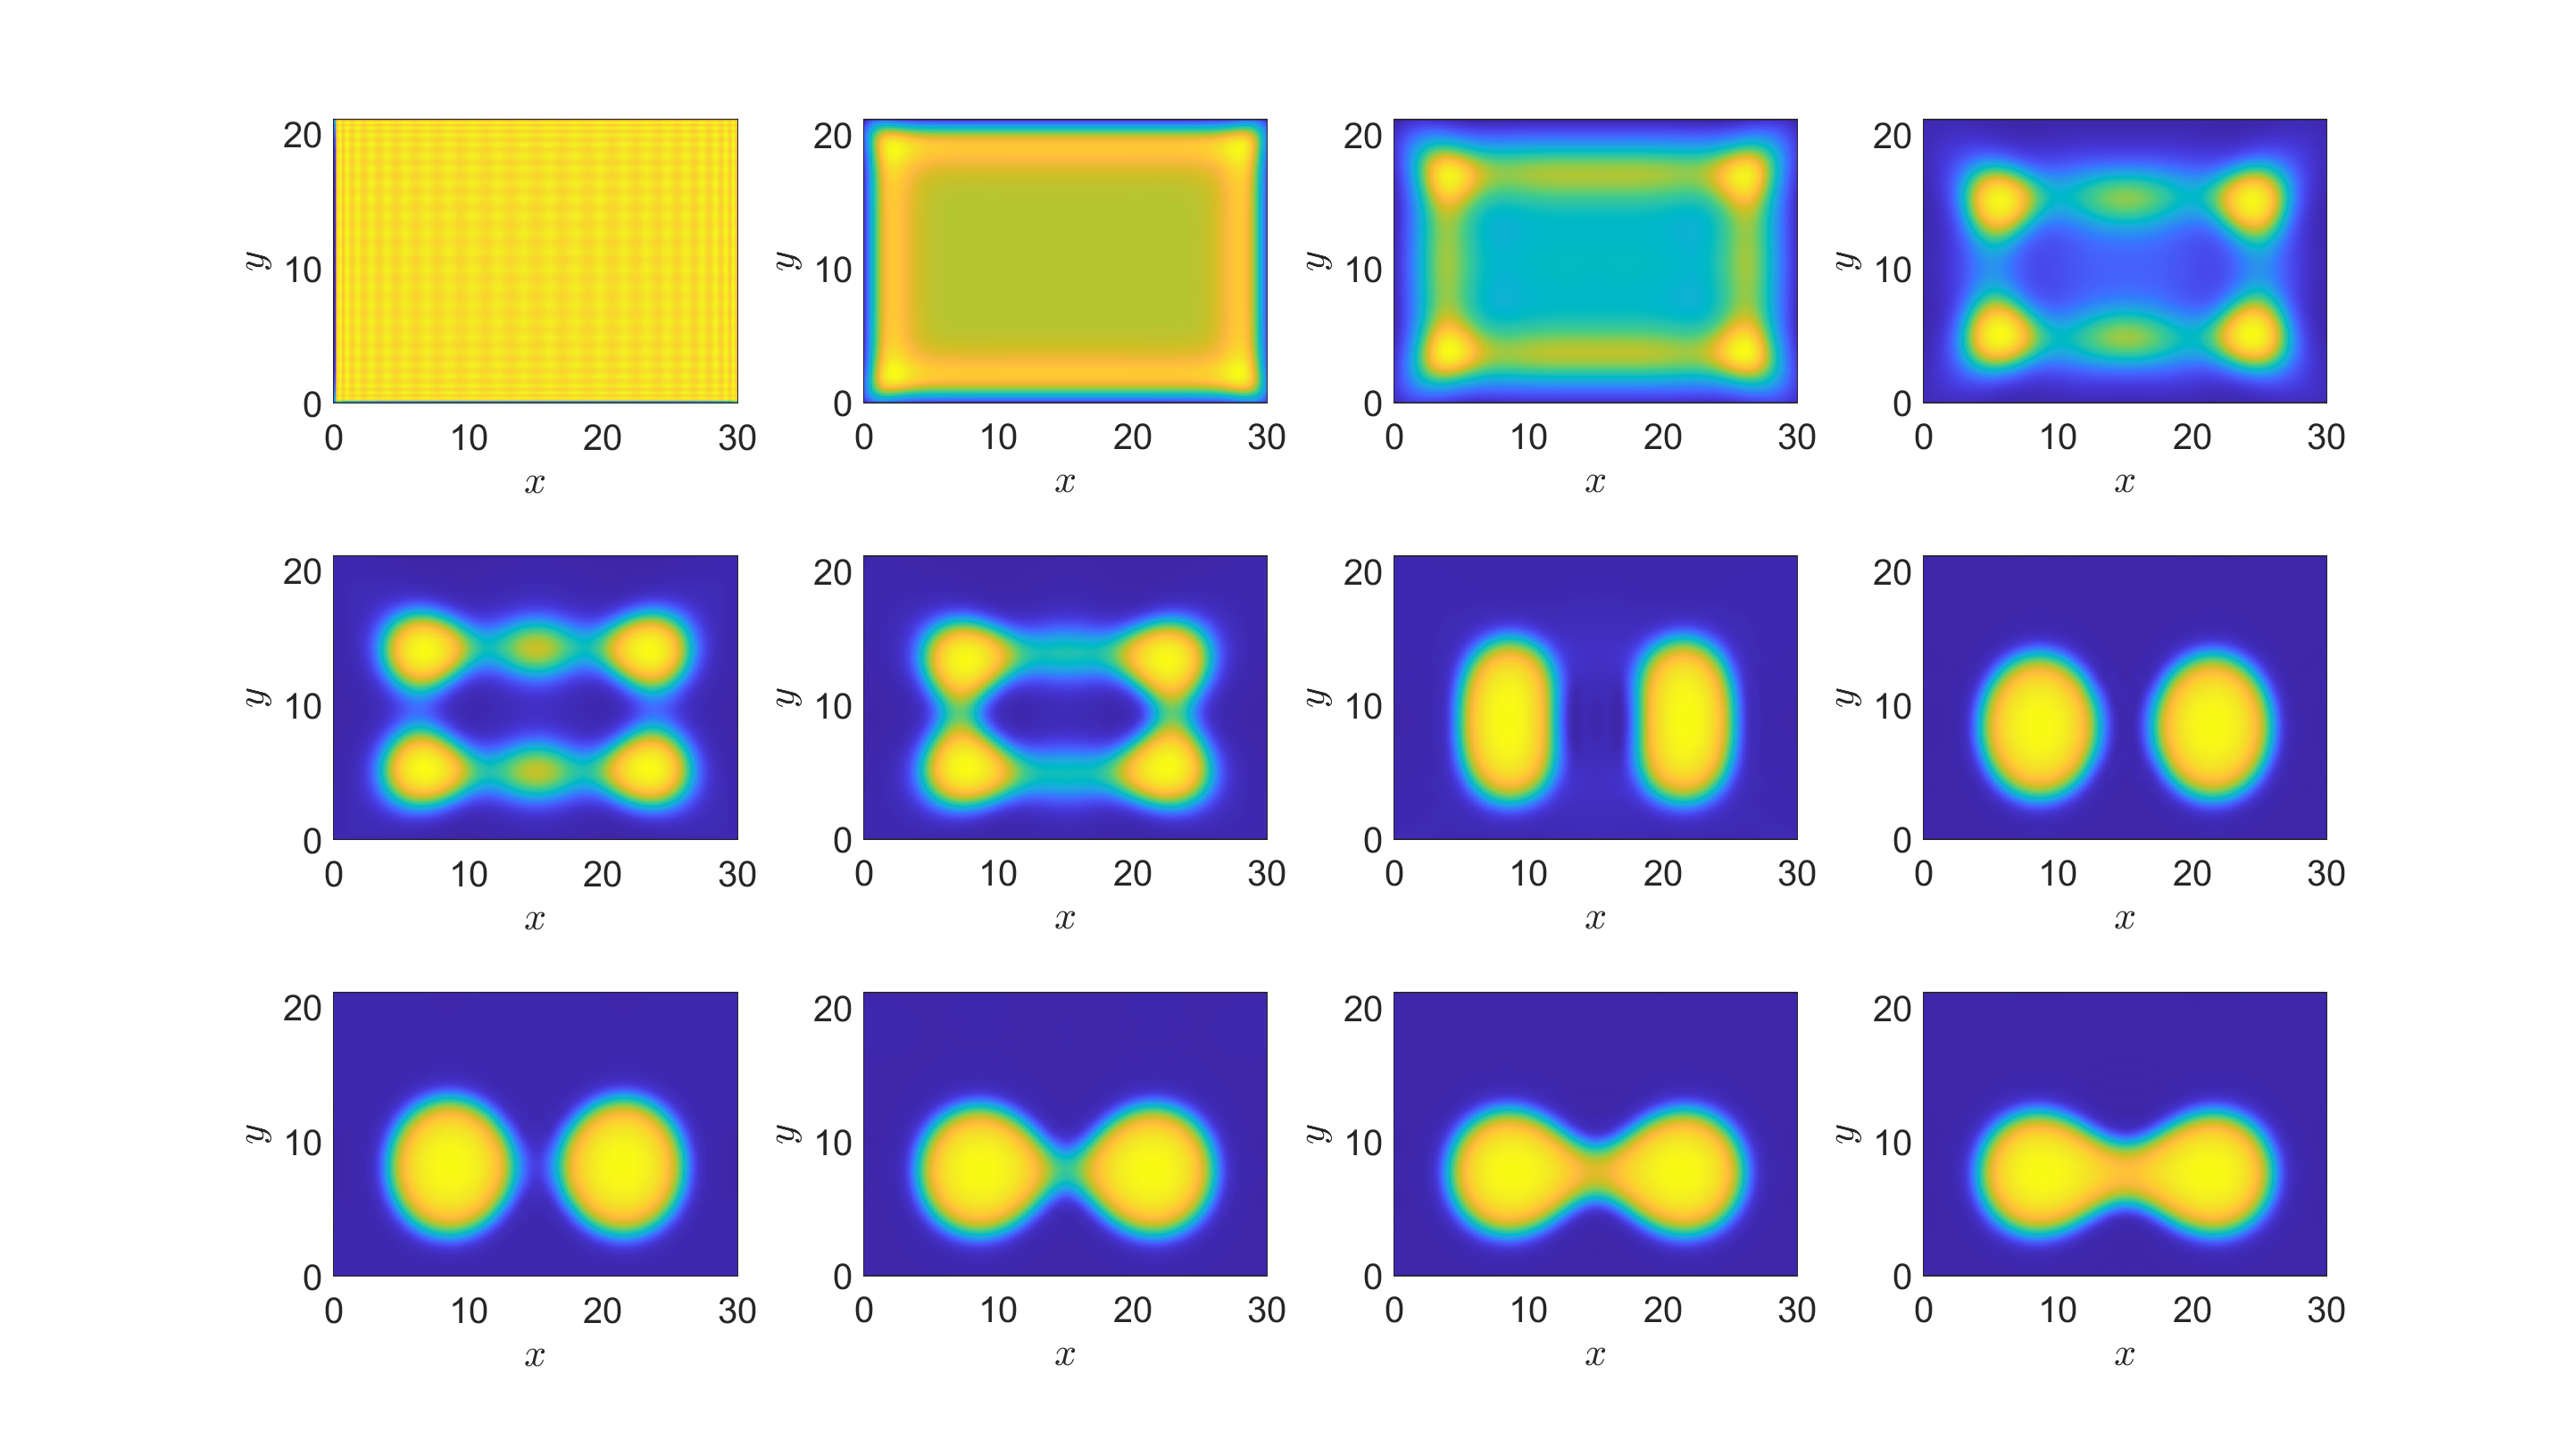
\includegraphics[scale=0.25]{Ex10F1.png}
		\caption{Figure 10 Example, $\bar \rho = 0.2$, $\sigma = 1$, $12$ different times} 
		\label{F4}
	\end{figure} 
	Again, since we have half of the original domain, we set $\sigma = 0.6$. We use $60$ points but that is not enough again as can be seen in Figure \ref{F4a}.
	\begin{figure}[h]
		\centering
		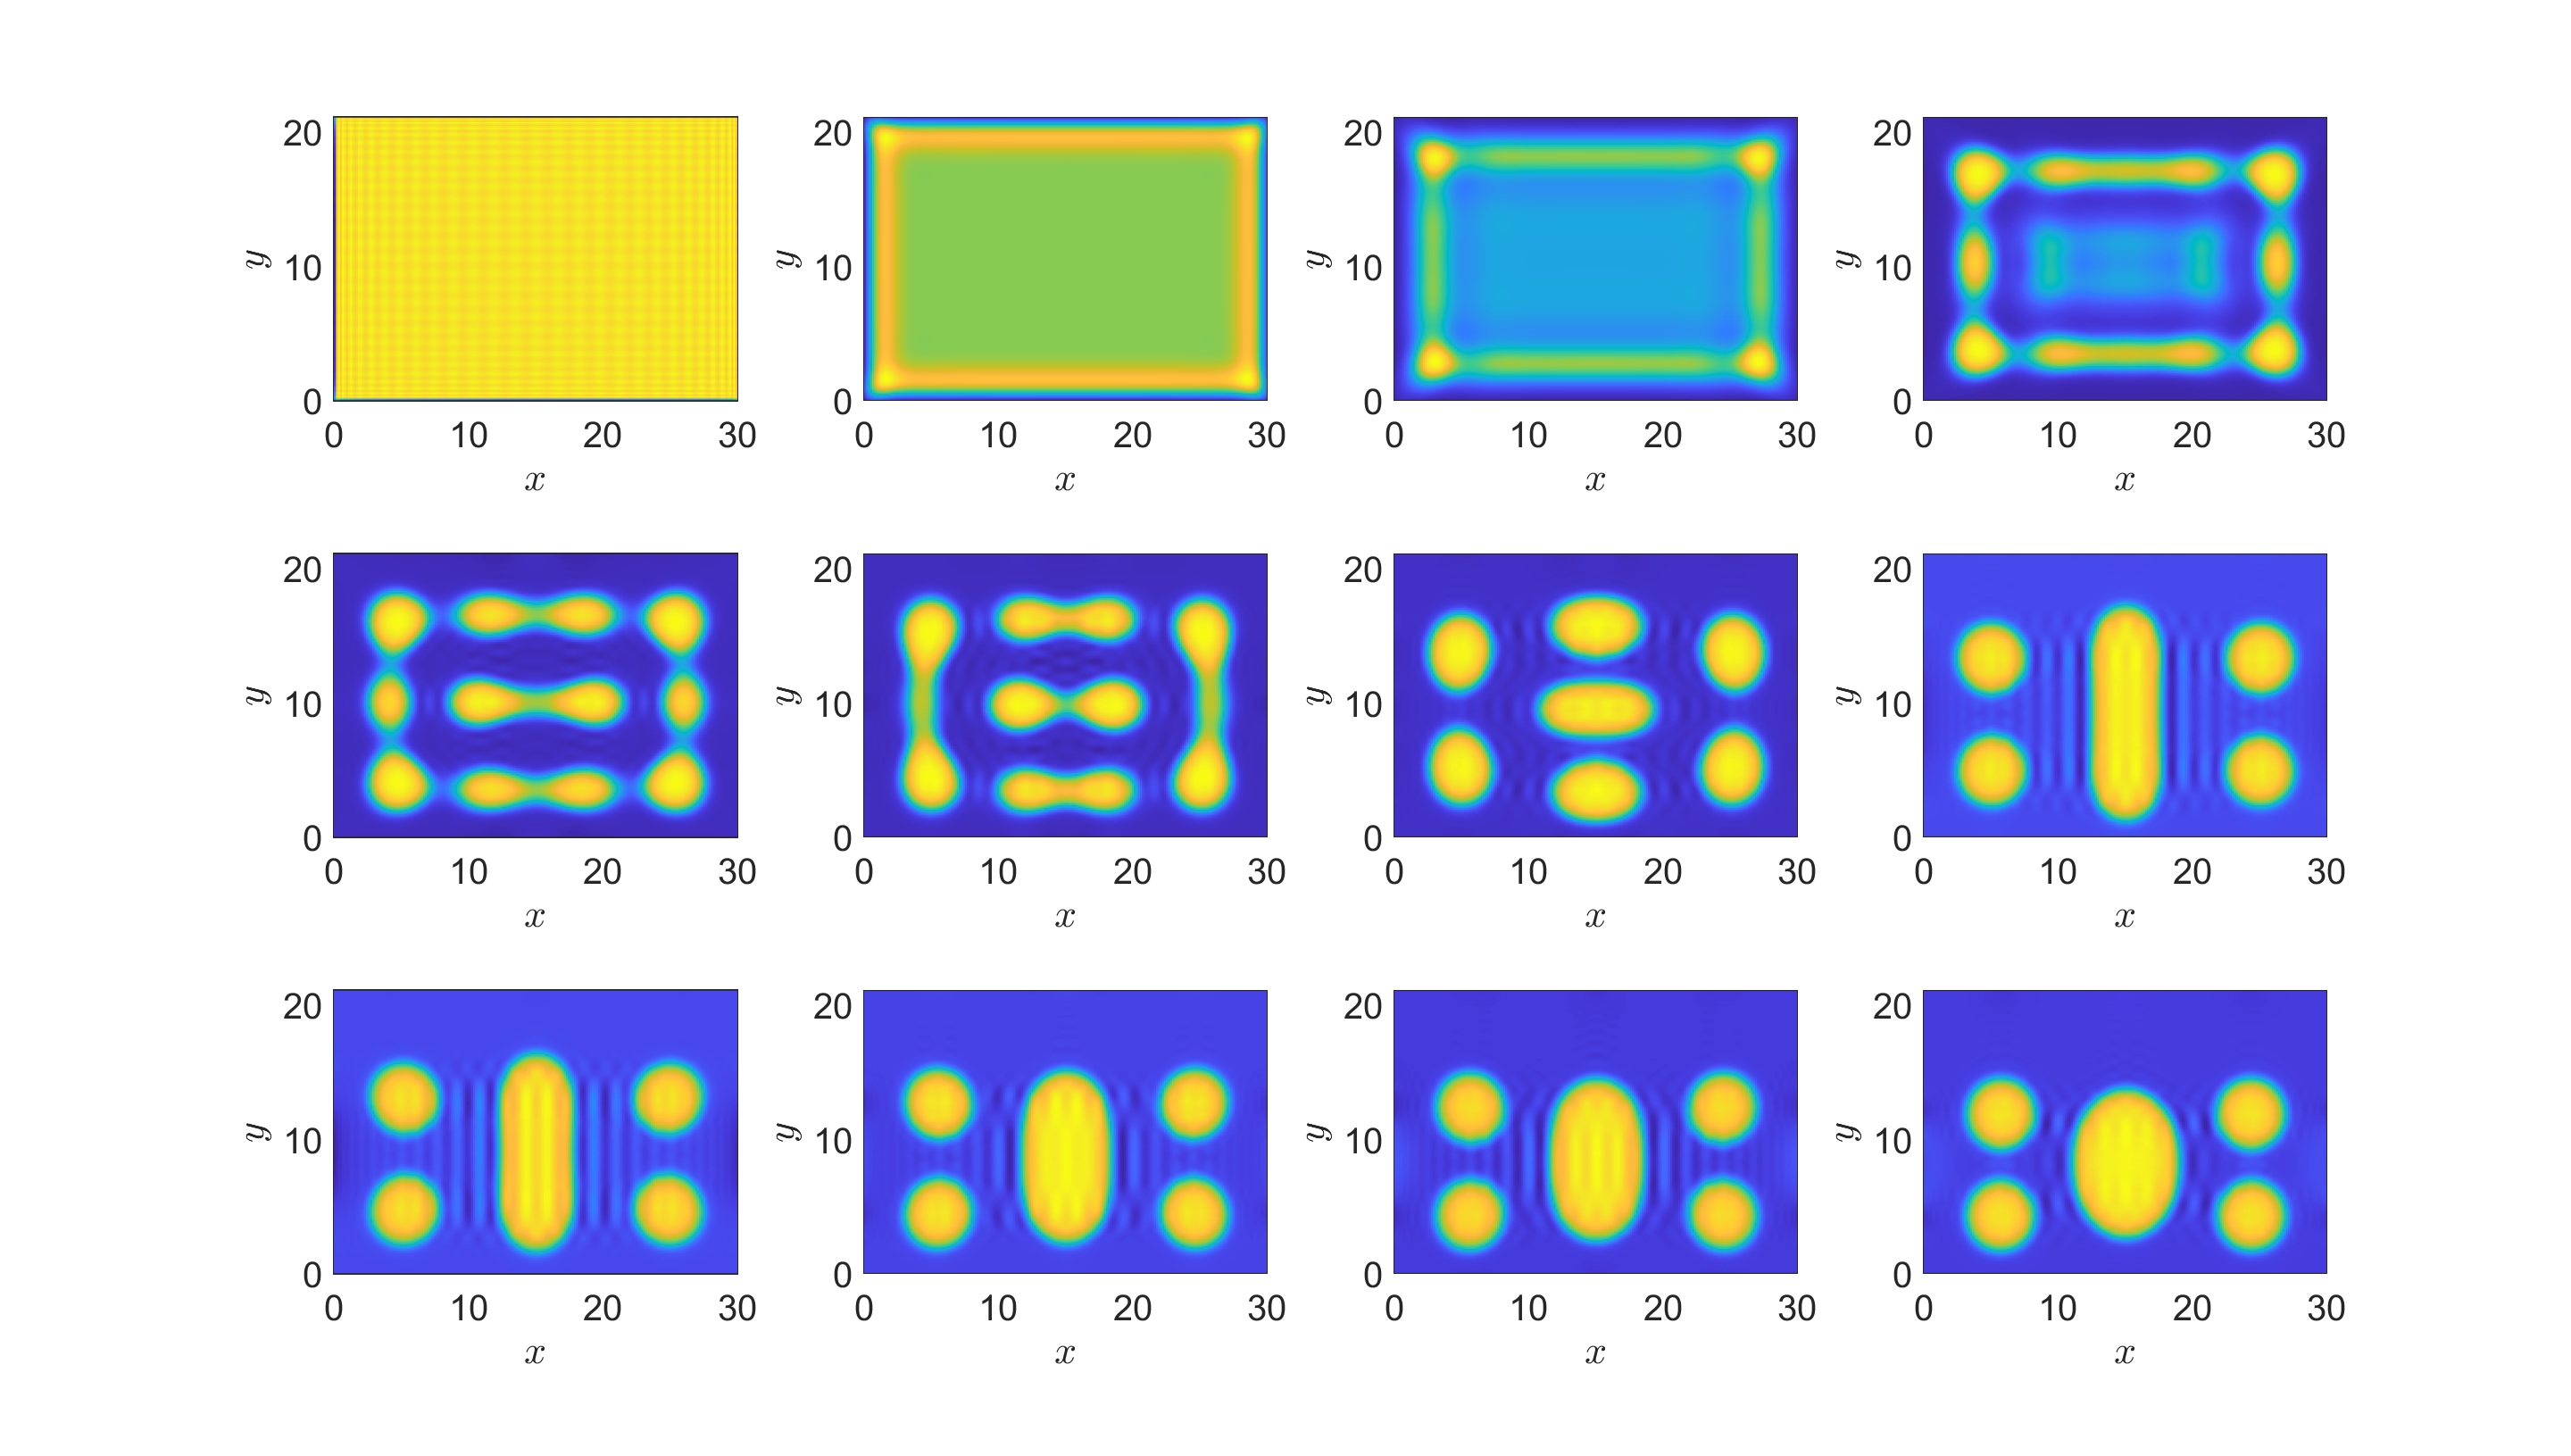
\includegraphics[scale=0.25]{Ex10F2.png}
		\caption{Figure 10 Example, $\bar \rho = 0.2$, $\sigma = 0.6$, $12$ different times} 
		\label{F4a}
	\end{figure} 
	
	\section{Replicating examples from the paper in a periodic box}
	Since the original simulations are done in a periodic box, we implement the problem in the periodic box as well. We expect near identical results to the paper, given that the setup is now identical.
	We choose a periodic box that has no flux boundary conditions on the top and bottom of the box, while being periodic on the sides. 
	We scale time as done in Equation \eqref{Eq1}, so that the time scales are comparable. In order to get qualitatively good results, we choose $n =100$ and $N = 100$. This takes approximately five hours to solve. In Figures \ref{F5} and \ref{F6} the results for the configurations corresponding to Figure 8 in Archer's paper can be seen ($ \bar \rho = 0.072$, choosing $\sigma = 1$, and running up to $T = 300$). In Figures \ref{F7} and \ref{F8} we see the results that correspond to the configurations in Figure 10 in Archer's paper ($ \bar \rho = 0.2$, choosing $\sigma = 1$, running time up to $T = 300$). While the results for Archer's first result look very close to the original, the second set of results is a little different. This may have to do with slightly different initial conditions or numerical solutions.
	

	\begin{figure}[h]
		\centering
		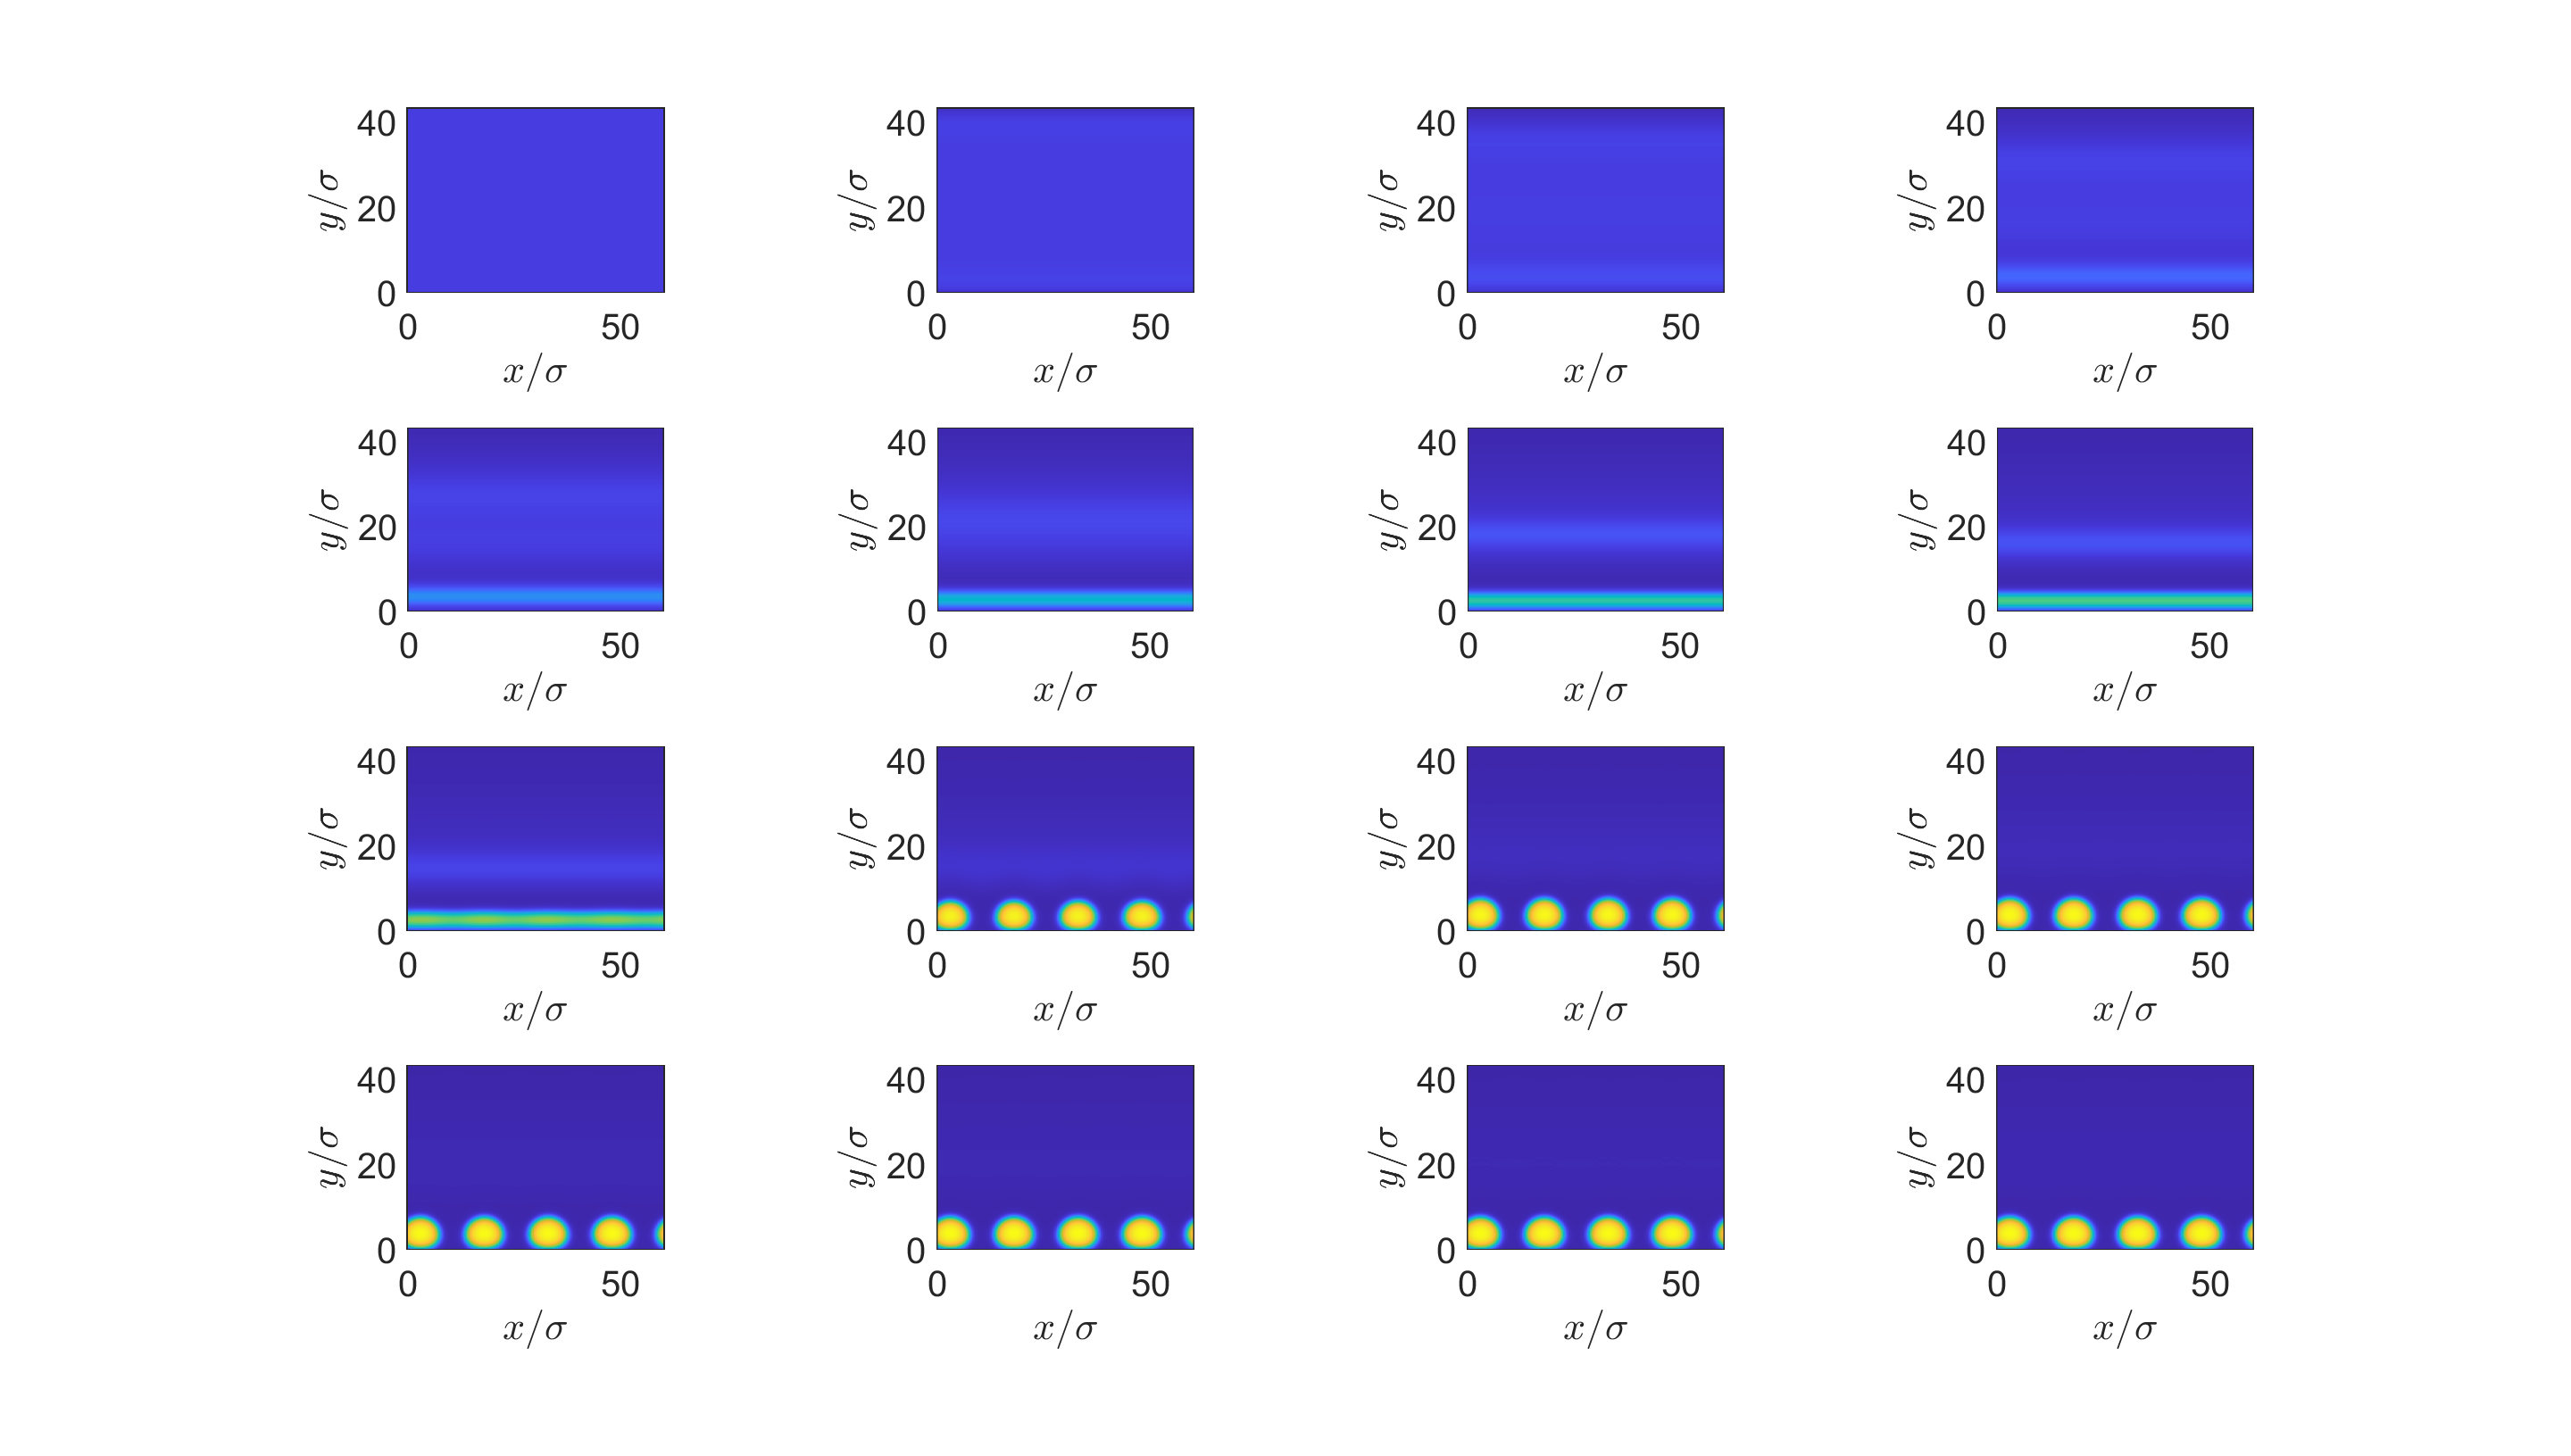
\includegraphics[scale=0.25]{Plotrhobar0072.png}
		\caption{Figure 8 in paper, result at each time} 
		\label{F5}
	\end{figure}
	\begin{figure}[h]
		\centering
		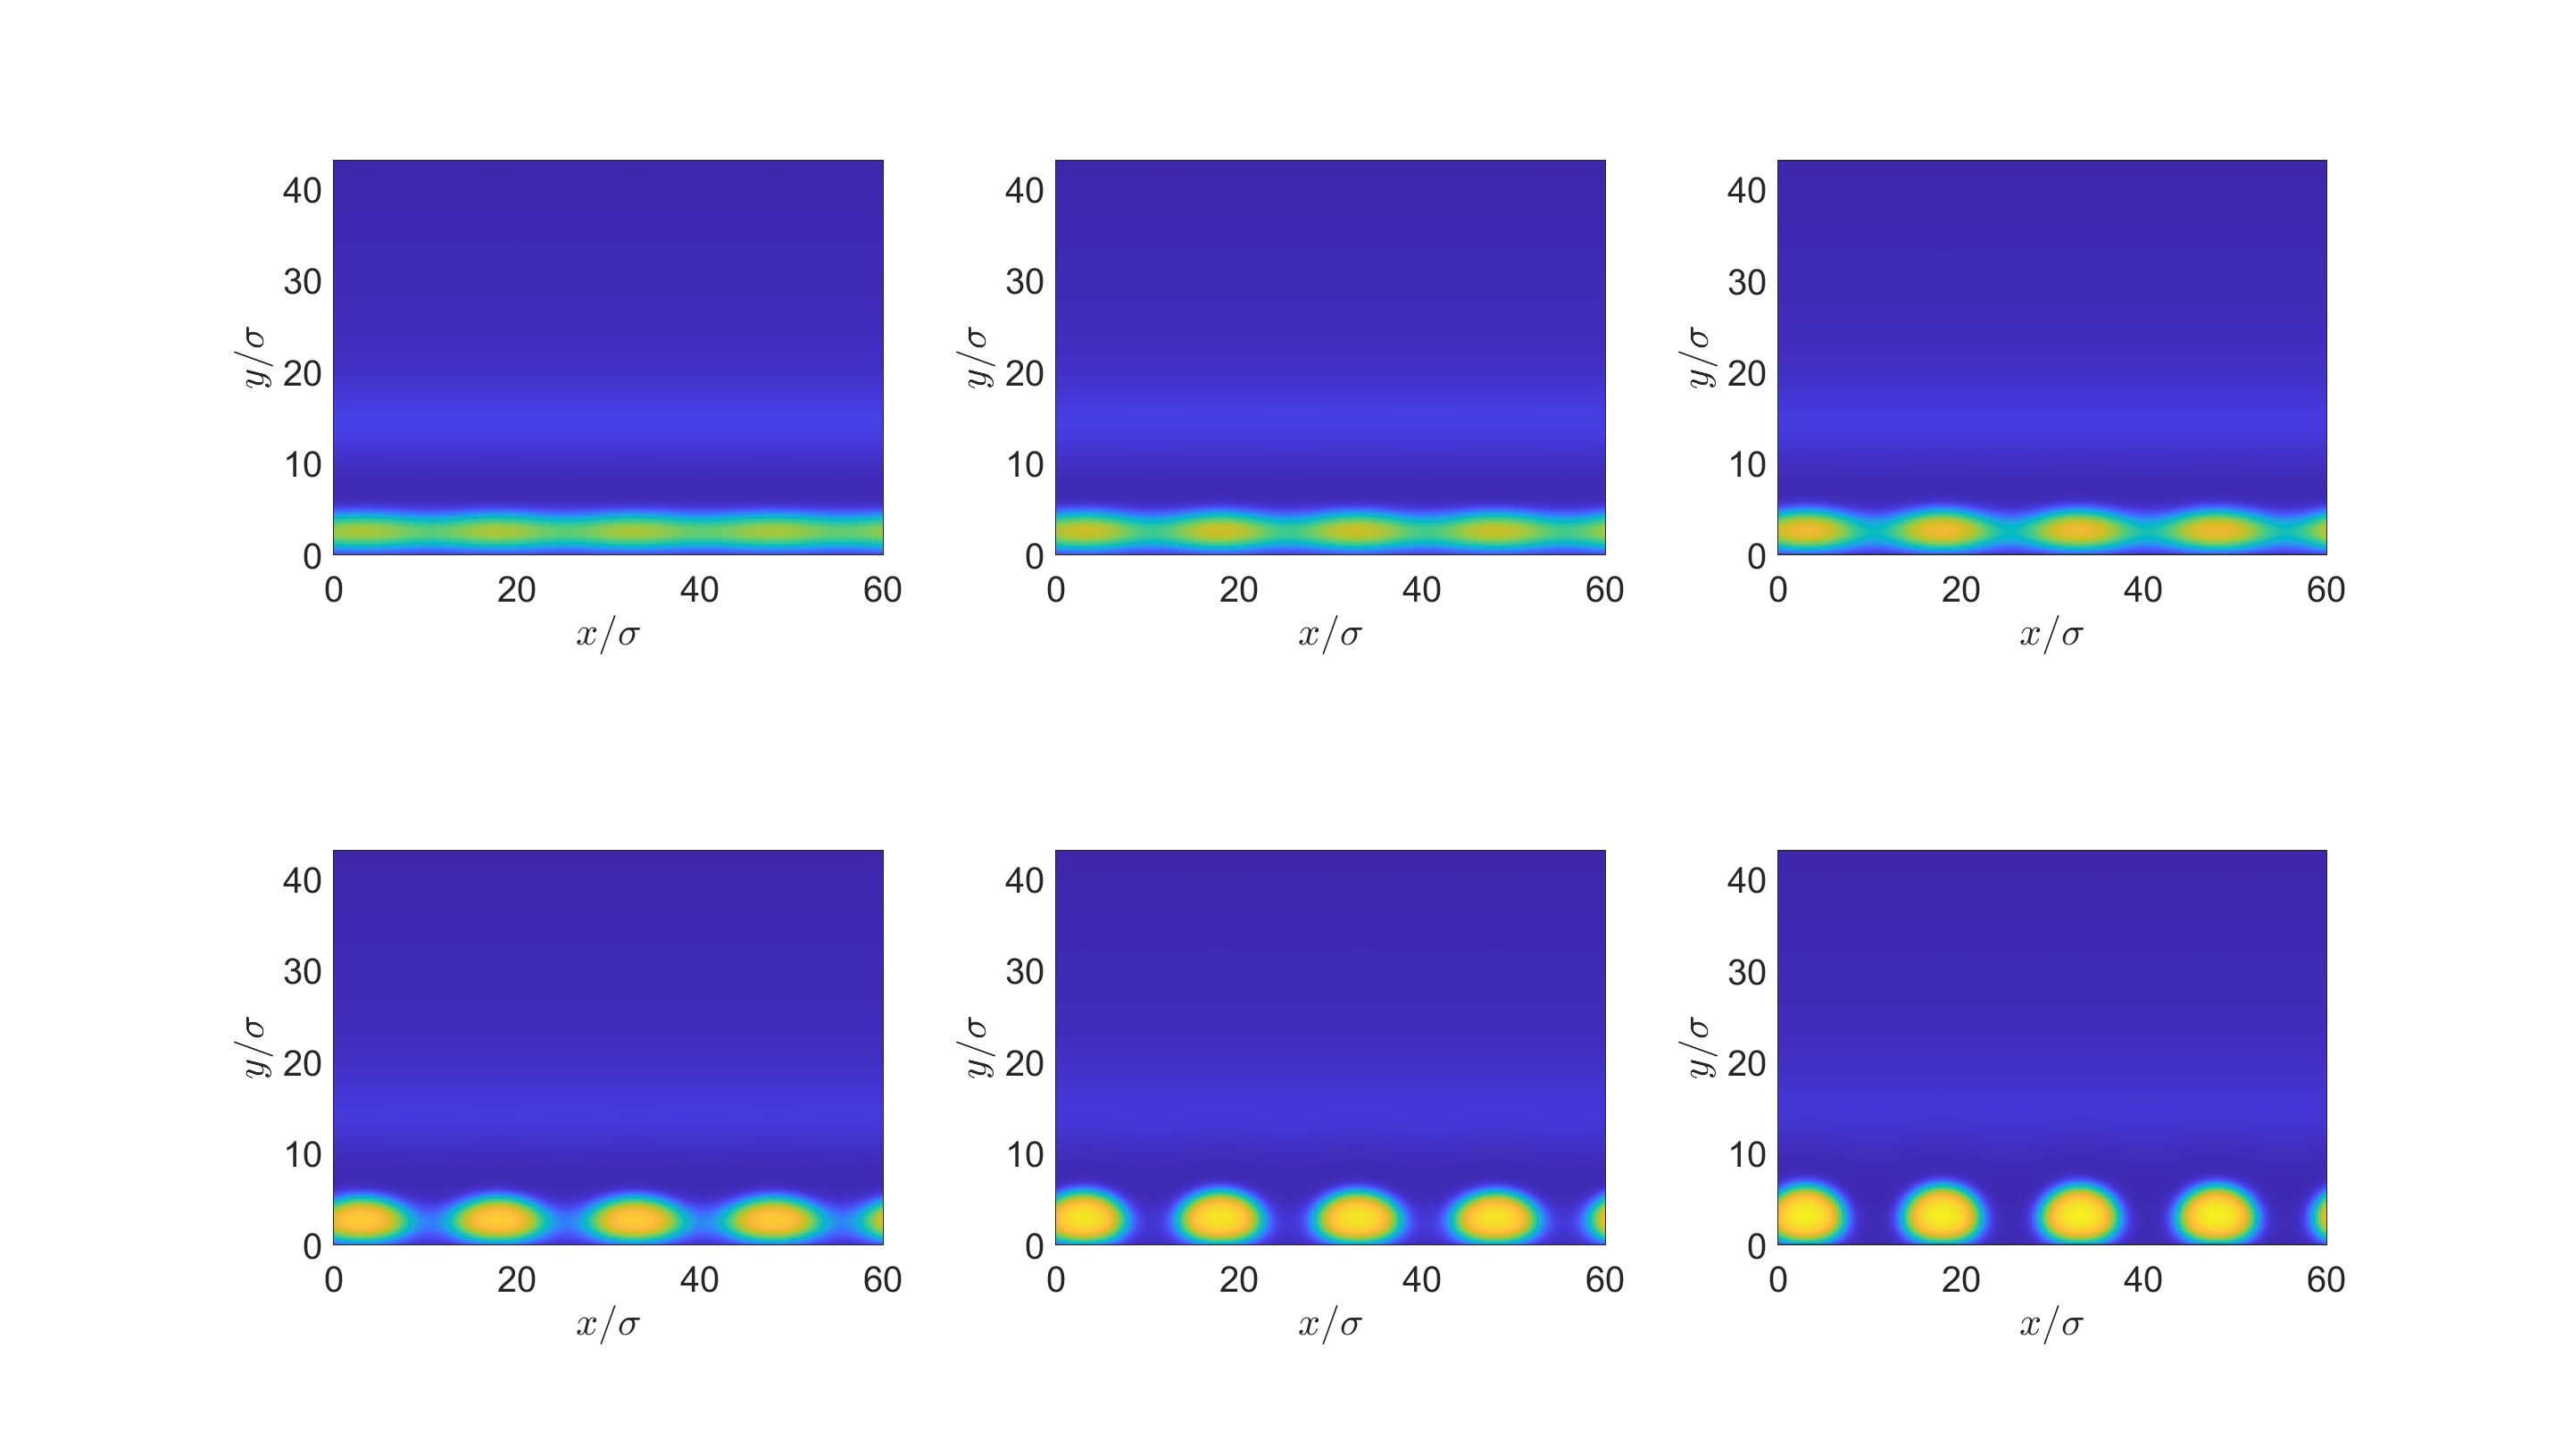
\includegraphics[scale=0.25]{rhobar0072Zoom57to62.png}
		\caption{Figure 8 in paper, result at times 57 - 62 out of 100} 
		\label{F6}
	\end{figure}

	\begin{figure}[h]
		\centering
		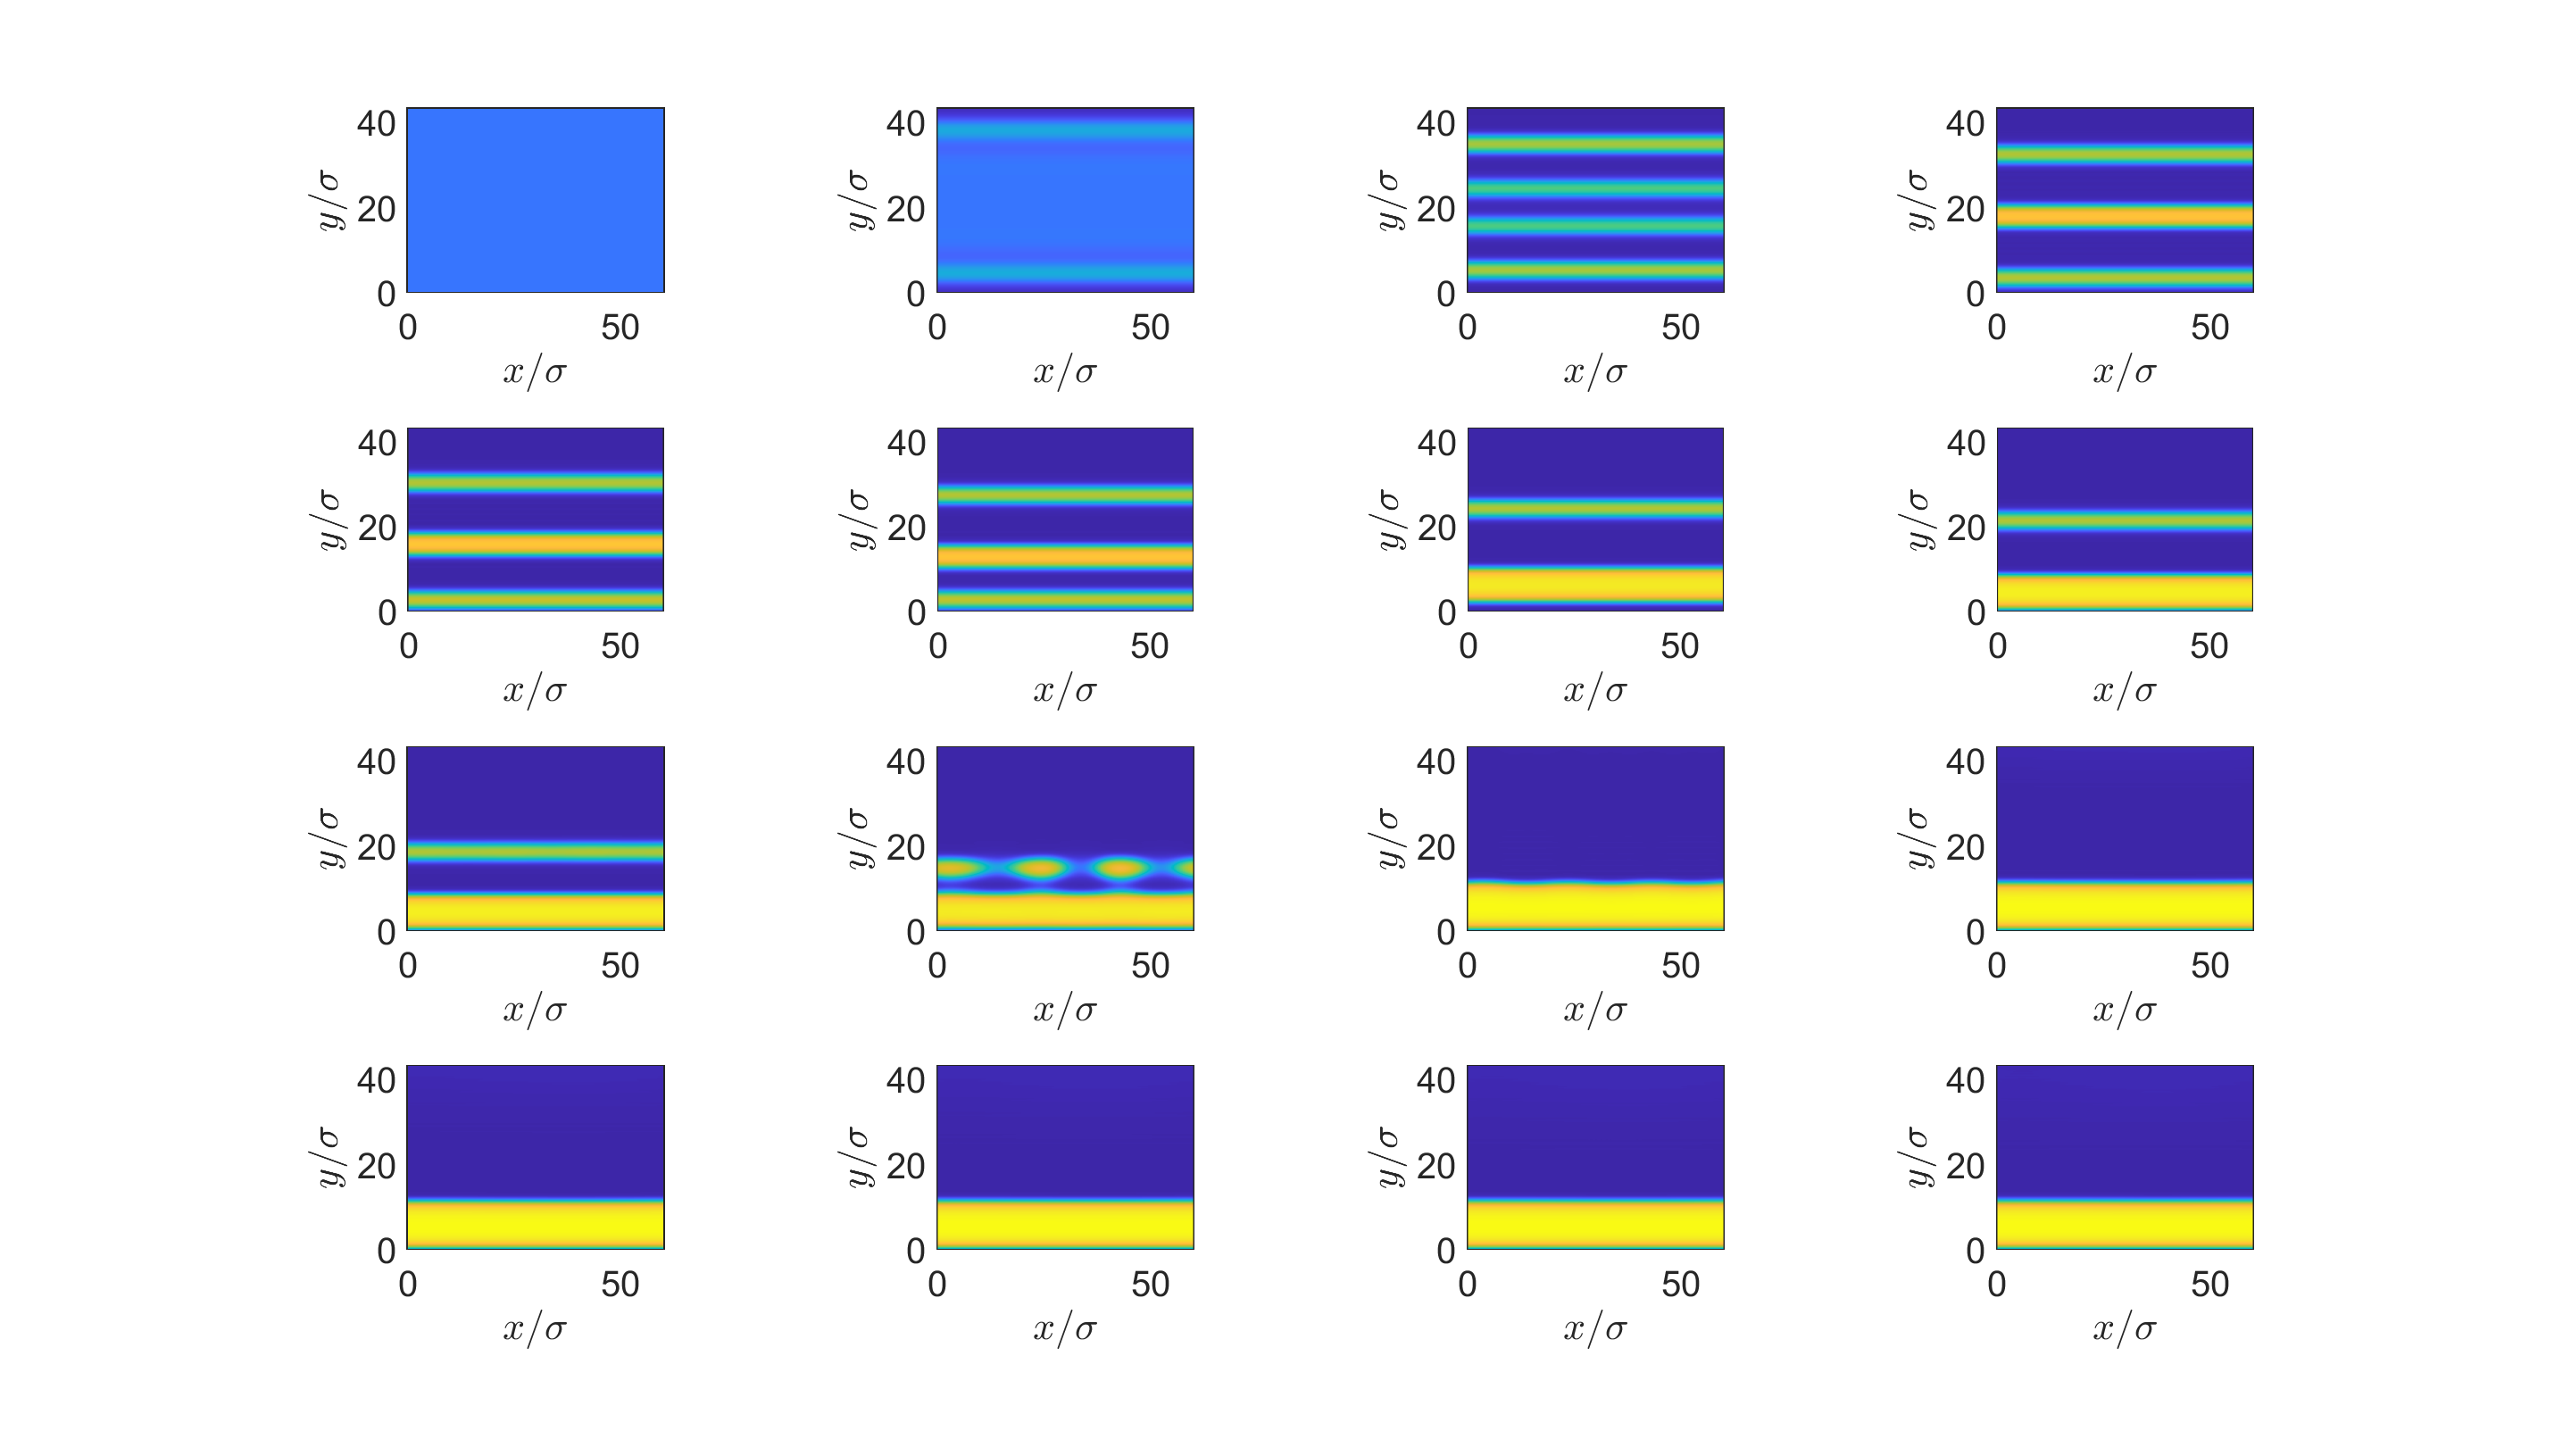
\includegraphics[scale=0.25]{Plotrhobar02.png}
		\caption{Figure 10 in paper, result at each time} 
		\label{F7}
	\end{figure}
	\begin{figure}[h]
		\centering
		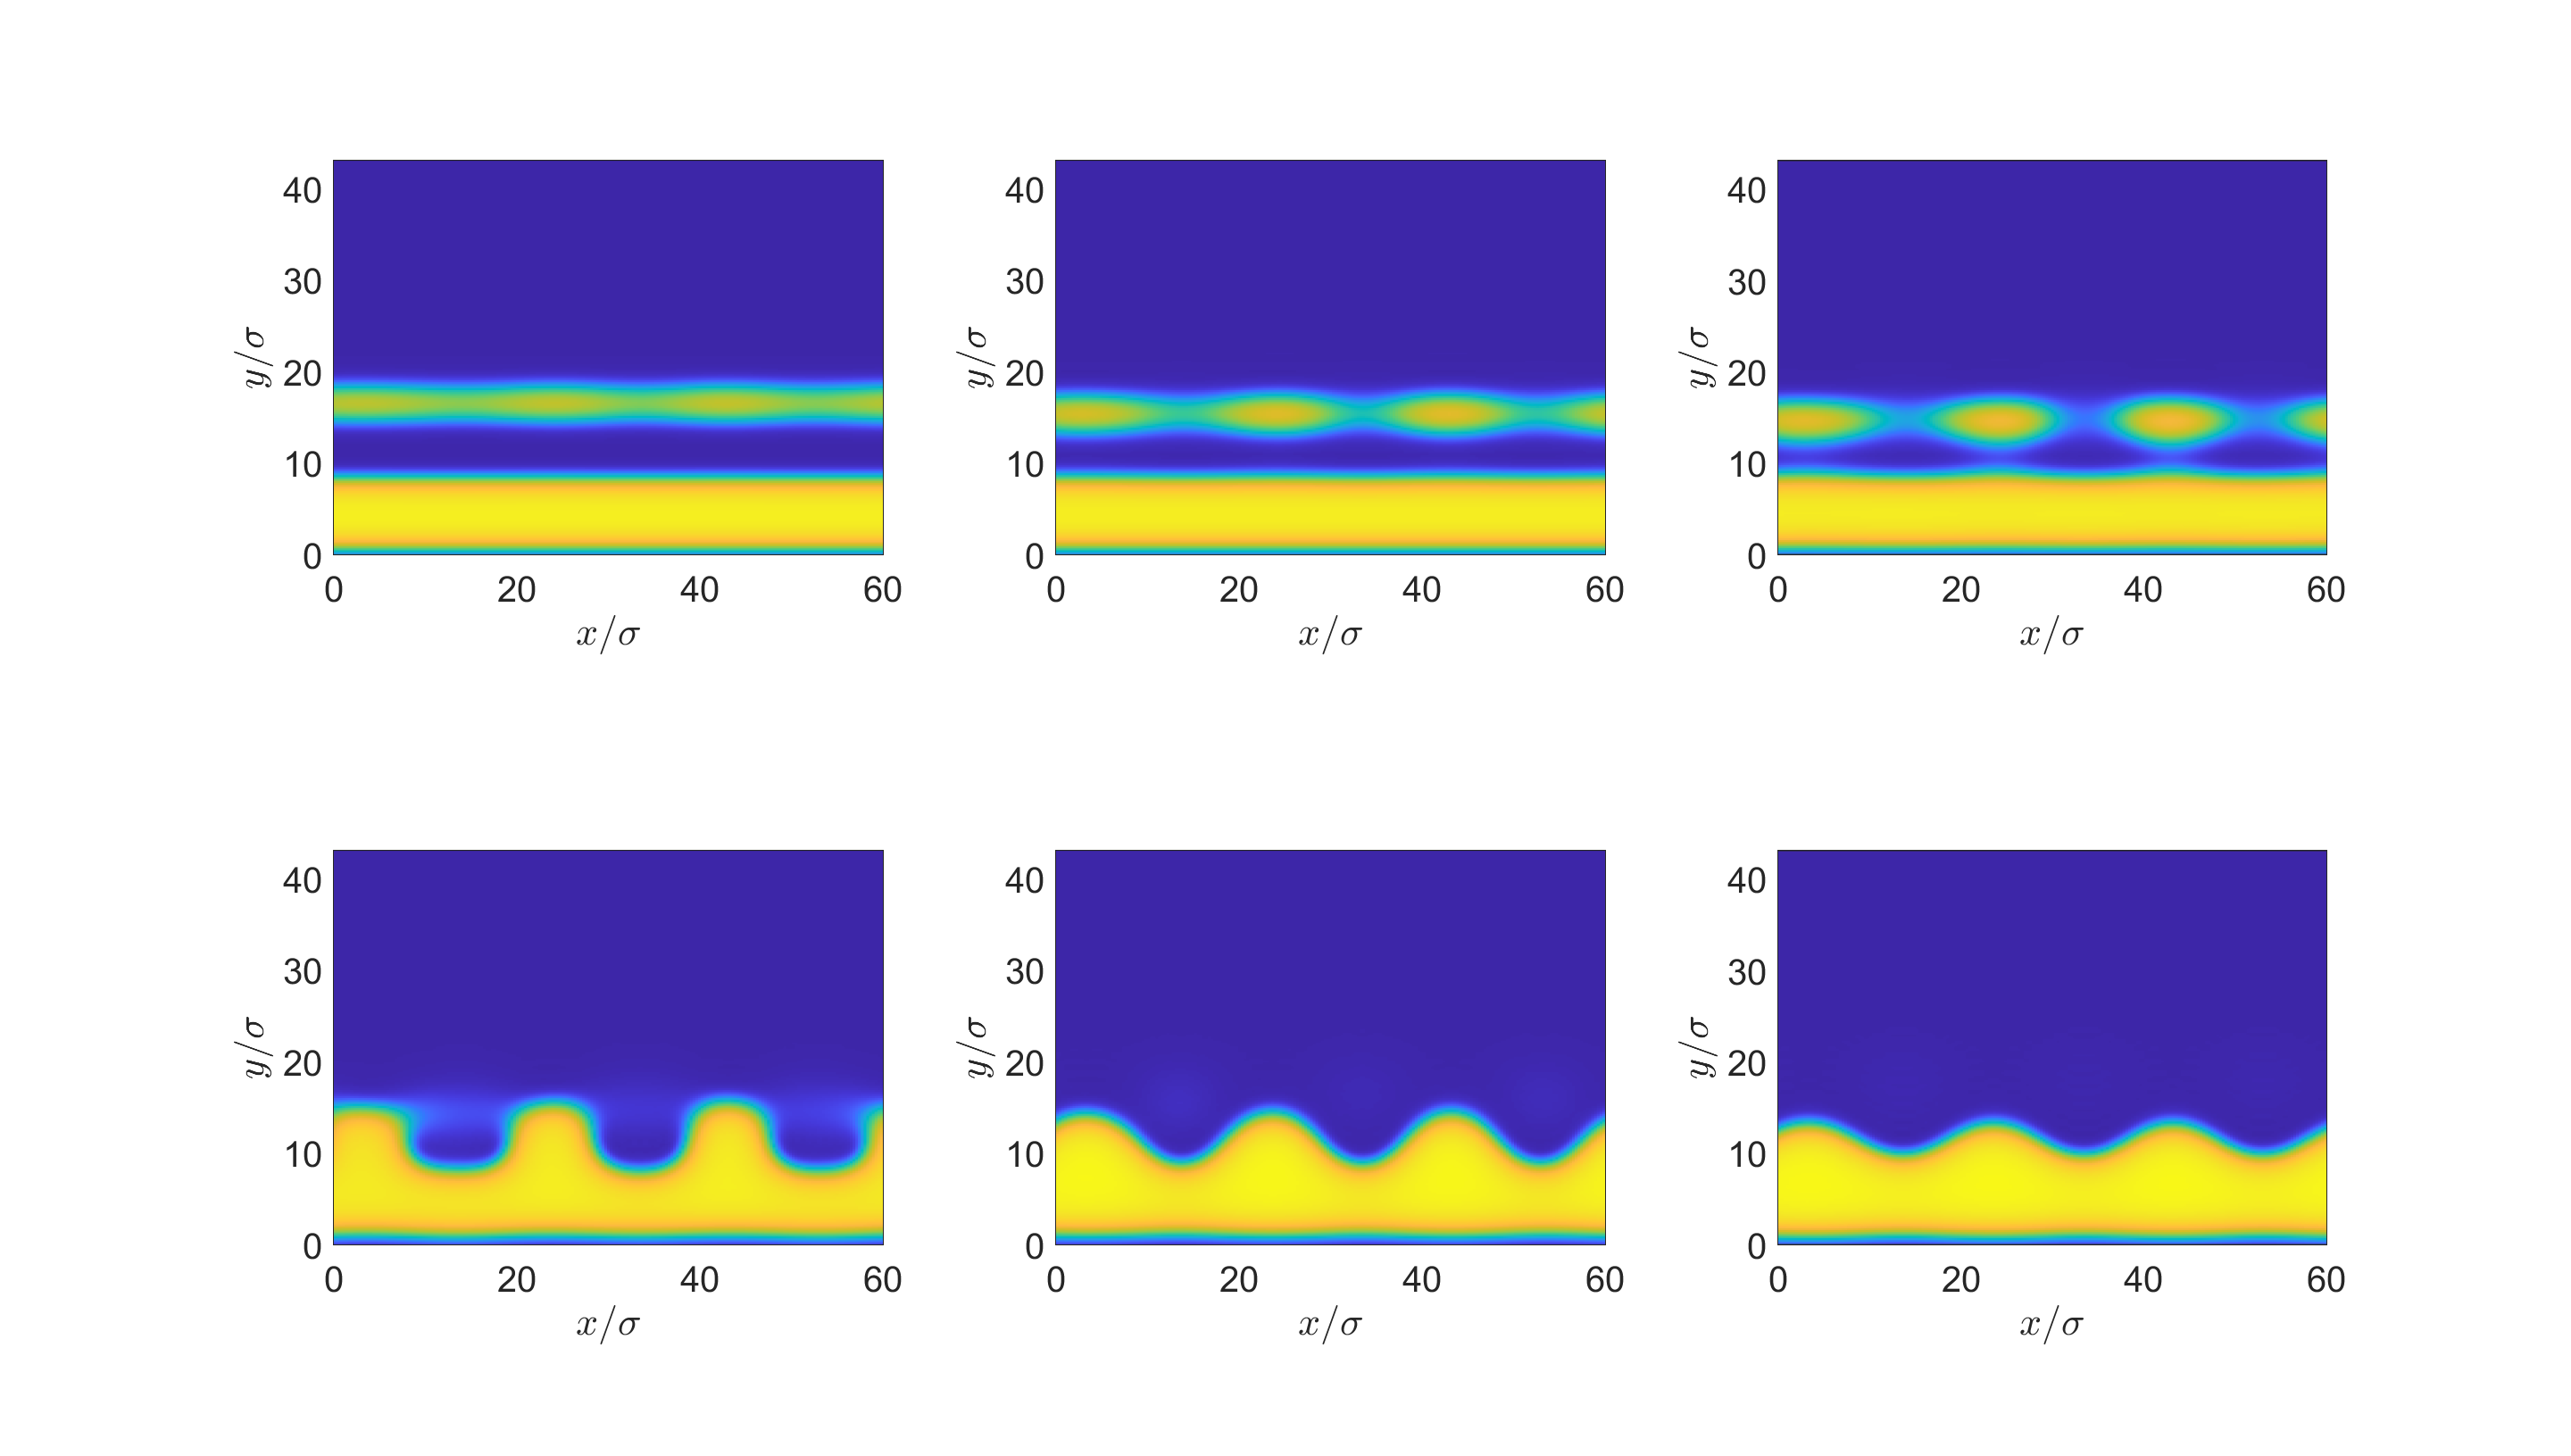
\includegraphics[scale=0.25]{rhobar02Zoom60to66.png}
		\caption{Figure 8 in paper, result at times 60 - 66 out of 100} 
		\label{F8}
	\end{figure}
	\section{Reference}
	Andrew J. Archer \& Alexandr Malijevský (2011) On the interplay between sedimentation and phase separation phenomena in two-dimensional colloidal fluids, Molecular Physics, 109:7-10, 1087-1099, DOI: 10.1080/00268976.2010.544267
\end{document}